\documentclass[12pt,a4paper]{article}
\usepackage[left=2cm,right=2cm,top=2cm,bottom=2cm]{geometry}
\usepackage[utf8]{inputenc}
\usepackage[T2A]{fontenc}
\usepackage{amsmath}
\usepackage{amssymb}
\usepackage{graphicx}
\usepackage[russian]{babel}
\usepackage{indentfirst}
\usepackage{listings}
\usepackage{xcolor}
\usepackage{hyperref}

\hypersetup{
  colorlinks=true,
  urlcolor= blue,
  citecolor=blue,
  linkcolor= blue,
}

\title{Отчет по лабораторным работам №1-6 по дисциплине
	"Математическая статистика"}
\author{Скворцов Владимир Сергеевич (5030102/10201)}
\date{\today}

\begin{document}

	\begin{titlepage}

		\Large

		\begin{center}
			Санкт-Петербургский \\ Политехнический университет Петра Великого

			\vspace{10em}

			\textbf{Отчет по лабораторным работам №1-6} \\
			\textbf{по дисциплине}\\
			"\textbf{Математическая статистика}"

			\vspace{2em}

		\end{center}

		\vspace{6em}

		\newbox{\lbox}
		\savebox{\lbox}{\hbox{Скворцов Владимир Сергеевич}}
		\newlength{\maxl}
		\setlength{\maxl}{\wd\lbox}
		\hfill\parbox{12cm}{
			\hspace*{3cm}\hspace*{-5cm}Студент:\hfill\hbox to\maxl{Скворцов Владимир Сергеевич\hfill}\\
			\hspace*{3cm}\hspace*{-5cm}Преподаватель:\hfill\hbox to\maxl{Баженов Александр Николаевич}\\
			\\
			\hspace*{3cm}\hspace*{-5cm}Группа:\hfill\hbox to\maxl{5030102/10201}\\
		}

		\vspace{\fill}

		\begin{center}
			Санкт-Петербург \\ 2024
		\end{center}

	\end{titlepage}

	\tableofcontents\newpage

	\section{Постановка задачи}

	\subsection{Описательная статистика}

	Для 5 распределений:

	\begin{itemize}
	\item Нормальное распределение \( N(x, 0, 1) \)
	\item распределение Коши \( C(x, 0, 1) \)
	\item Распределение Стьюдента \( t(x, 0, 3) \) с тремя степенями свободы
	\item Распределение Пуассона \( P(k, 10) \)
	\item Равномерное распределение \( U(x, -\sqrt3, \sqrt3) \)
	\end{itemize}

	Сгенерировать выборки размером 10, 50, 1000 элементов.
	Построить на одном рисунке гистограмму и график плотности распределения.

	\subsection{Точечное оценивание характеристик положения и рассеяния}

	Сгенерировать выборки размером 10, 50, 1000 элементов.
	Для каждой выборки вычислить следующие статистические характеристики
	положения данных: \( \overline{x} \), \( med\:x \), \( z_{Q} \), \( z_{R} \),
	\( z_{tr} \). Повторить такие вычисления 1000 раз для каждой выборки и
	найти среднее характеристик положения и их квадратов:
	\( E(z) = \bar{z} \). Вычислить оценку дисперсии по формуле
	\( D(z) = \overline{z^2} - \overline{z}^2 \).

	\section{Теоретическое обоснование}
	\subsection{Функции распределения}
	\begin{itemize}
		\item Нормальное распределение

		\begin{equation} \label{eq:normal}
			N(x, 0, 1) = \frac{1}{\sqrt{2\pi}}e^\frac{-x^2}{2}
		\end{equation}

		\item Распределение Коши

		\begin{equation} \label{eq:cauchy}
			C(x, 0, 1) = \frac{1}{\pi}\frac{1}{x^2+1}
		\end{equation}

		\item Распределение Стьюдента \( t(x, 0, 3) \) с тремя степенями свободы

		\begin{equation} \label{eq:student}
			t(x, 0, 3) = \frac{6\sqrt3}{\pi(3 + t^2)^2}
		\end{equation}

		\item Распределение Пуассона

		\begin{equation} \label{eq:poisson}
			P(k, 10) = \frac{10^k}{k!}e^{-10}
		\end{equation}

		\item Равномерное распределение

		\begin{equation} \label{eq:uniform}
			U(x, -\sqrt3, \sqrt3) = \begin{cases}
				\frac{1}{2\sqrt3} & \mbox{при} \; |x| \leq \sqrt3\\
				0 & \mbox{при} \; |x| > \sqrt3
			\end{cases}
		\end{equation}
	\end{itemize}

	\subsection{Характеристики положения и рассеяния}

	\begin{itemize}
		\item Выборочное среднее

		\begin{equation} \label{eq:mean}
			\overline{x} = \tfrac{1}{n}\sum_{i = 1}^{n}x_i
		\end{equation}

		\item Выборочная медиана

		\begin{equation} \label{eq:median}
			med\ x = \left\{
			\begin{array}{ccl}
			x_{(l + 1)} & \text{при} & n = 2l + 1\\
			\dfrac{x_{(l)} + x_{(l + 1)}}{2} & \text{при} & n = 2l
			\end{array}
			\right.
		\end{equation}

		\item Полусумма экстремальных выборочных элементов

		\begin{equation} \label{eq:half_sum_of_extremal_elements}
			z_{R} = \frac{x_{(1)} + x_{(n)}}{2}
		\end{equation}

		\item Полусумма квартилей \\
		Выборочная квартиль \( z_{p} \) порядка \( p \) определяется формулой

		\begin{equation} \label{eq:quartil}
			z_{p} = \left\{
			\begin{array}{ccl}
			x_{([np]+ 1)} & \text{при} & np\ \text{дробном}\\
			x_{(np)} & \text{при} & np\ \text{целом}
			\end{array}
			\right.
		\end{equation}

		Полусумма квартилей \\

		\begin{equation}  \label{eq:half_sum_of_quartiles}
			z_{Q} = \dfrac{z_{1/4} + z_{3/4}}{2}
		\end{equation}

		\item Усечённое среднее

		\begin{equation} \label{eq:trimmed_mean}
			z_{tr} = \tfrac{1}{n - 2r}\sum_{i = r + 1}^{n - r}x_{(i)},\
			r\approx\dfrac{n}{4}
		\end{equation}

		\item Среднее характеристики

		\begin{equation} \label{eq:expected_value}
			E(z) = \overline z
		\end{equation}

		\item Оценка дисперсии

		\begin{equation} \label{eq:dispersion}
			D(z) = \overline{z^2} - \overline{z}^2
		\end{equation}
	\end{itemize}

	\section{Описание работы}
	Лабораторные работы выполнены с использованием Python и его сторонних
	библиотек \verb!numpy!, \verb!pandas!, \verb!matplotlib!, \verb!seaborn! были
	построены гистограммы распределений и посчитаны характеристики пложения.

	Ссылка на GitHub репозиторий:
	\href{https://github.com/vladimir-skvortsov/spbstu-mathematical-statistics}
	{https://github.com/vladimir-skvortsov/spbstu-mathematical-statistics}

	\newpage

	\section{Результаты}

	\subsection{Гистограммы и графики плотности распределения}

	\begin{figure}[htbp!]
		\begin{center}
			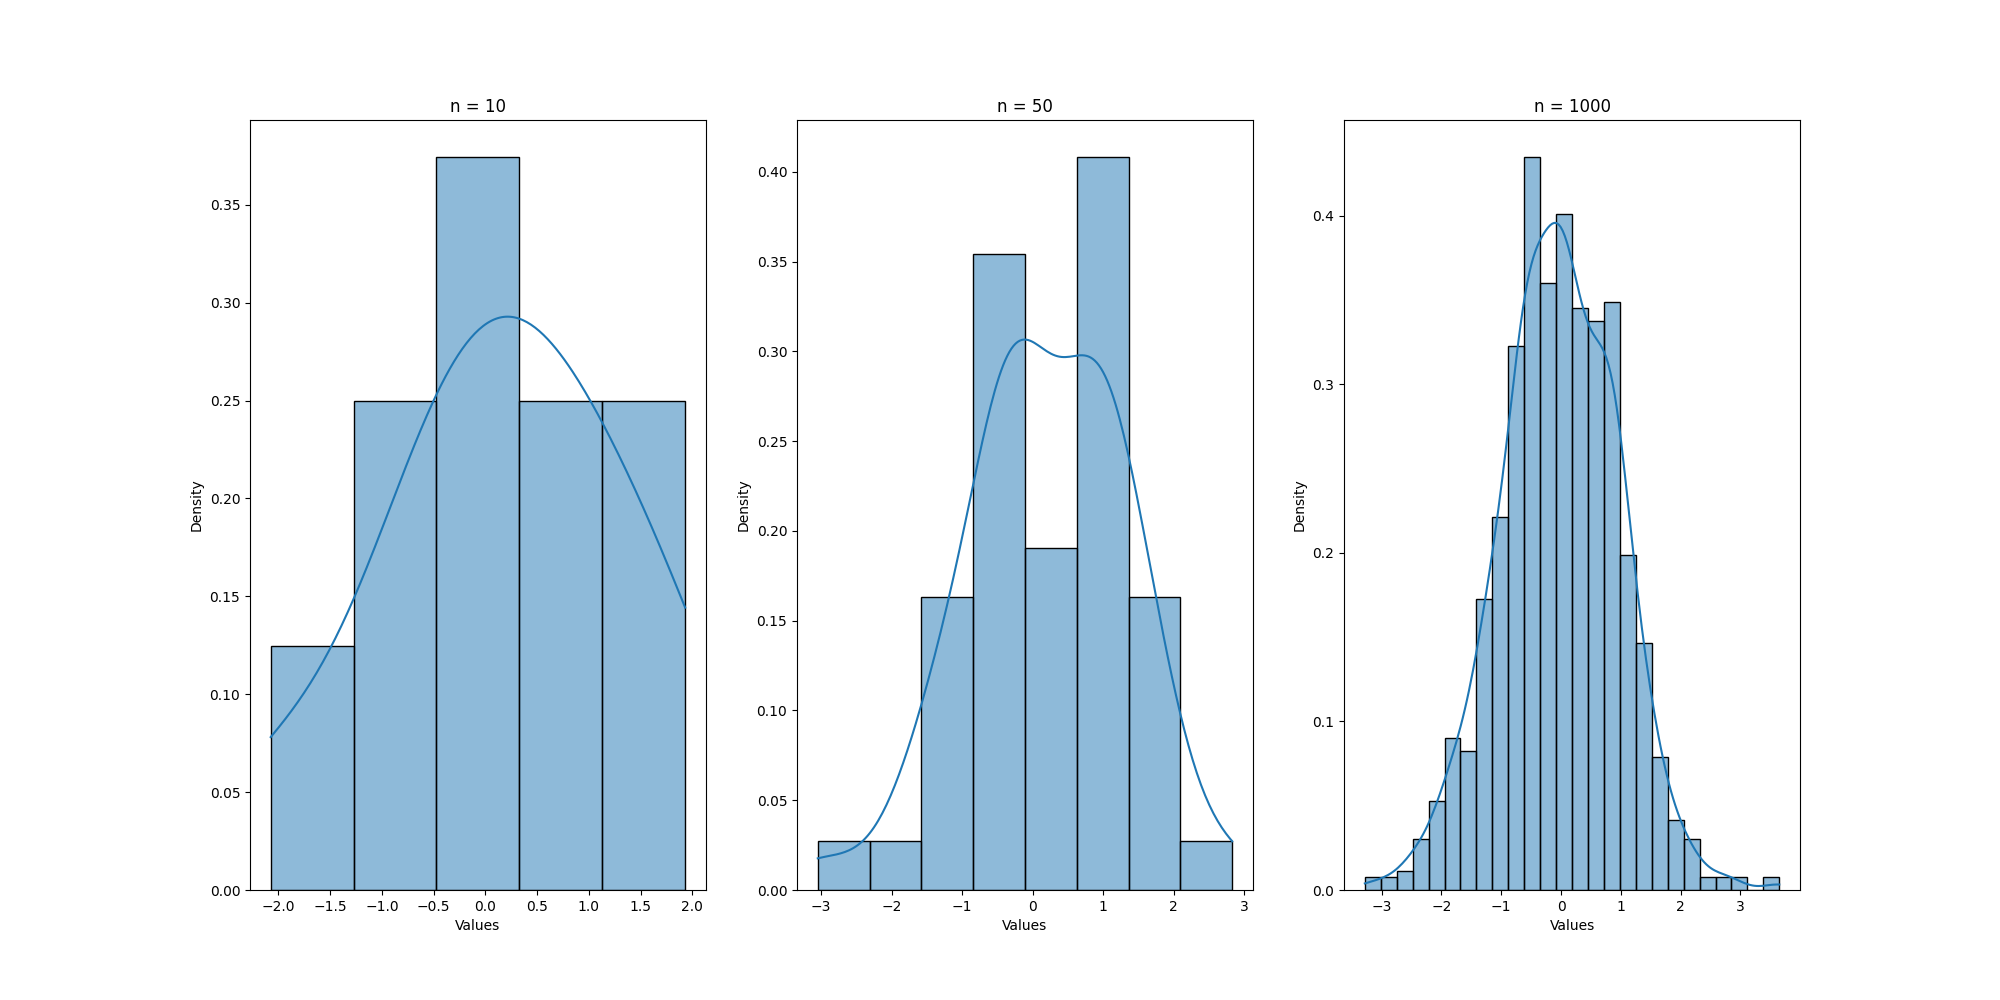
\includegraphics[width = 1.12\linewidth]{graphics/lab1_normal.png}
			\caption{Нормальное распределение \ \eqref{eq:normal}}
		\end{center}
	\end{figure}

	\begin{figure}[htbp!]
		\begin{center}
			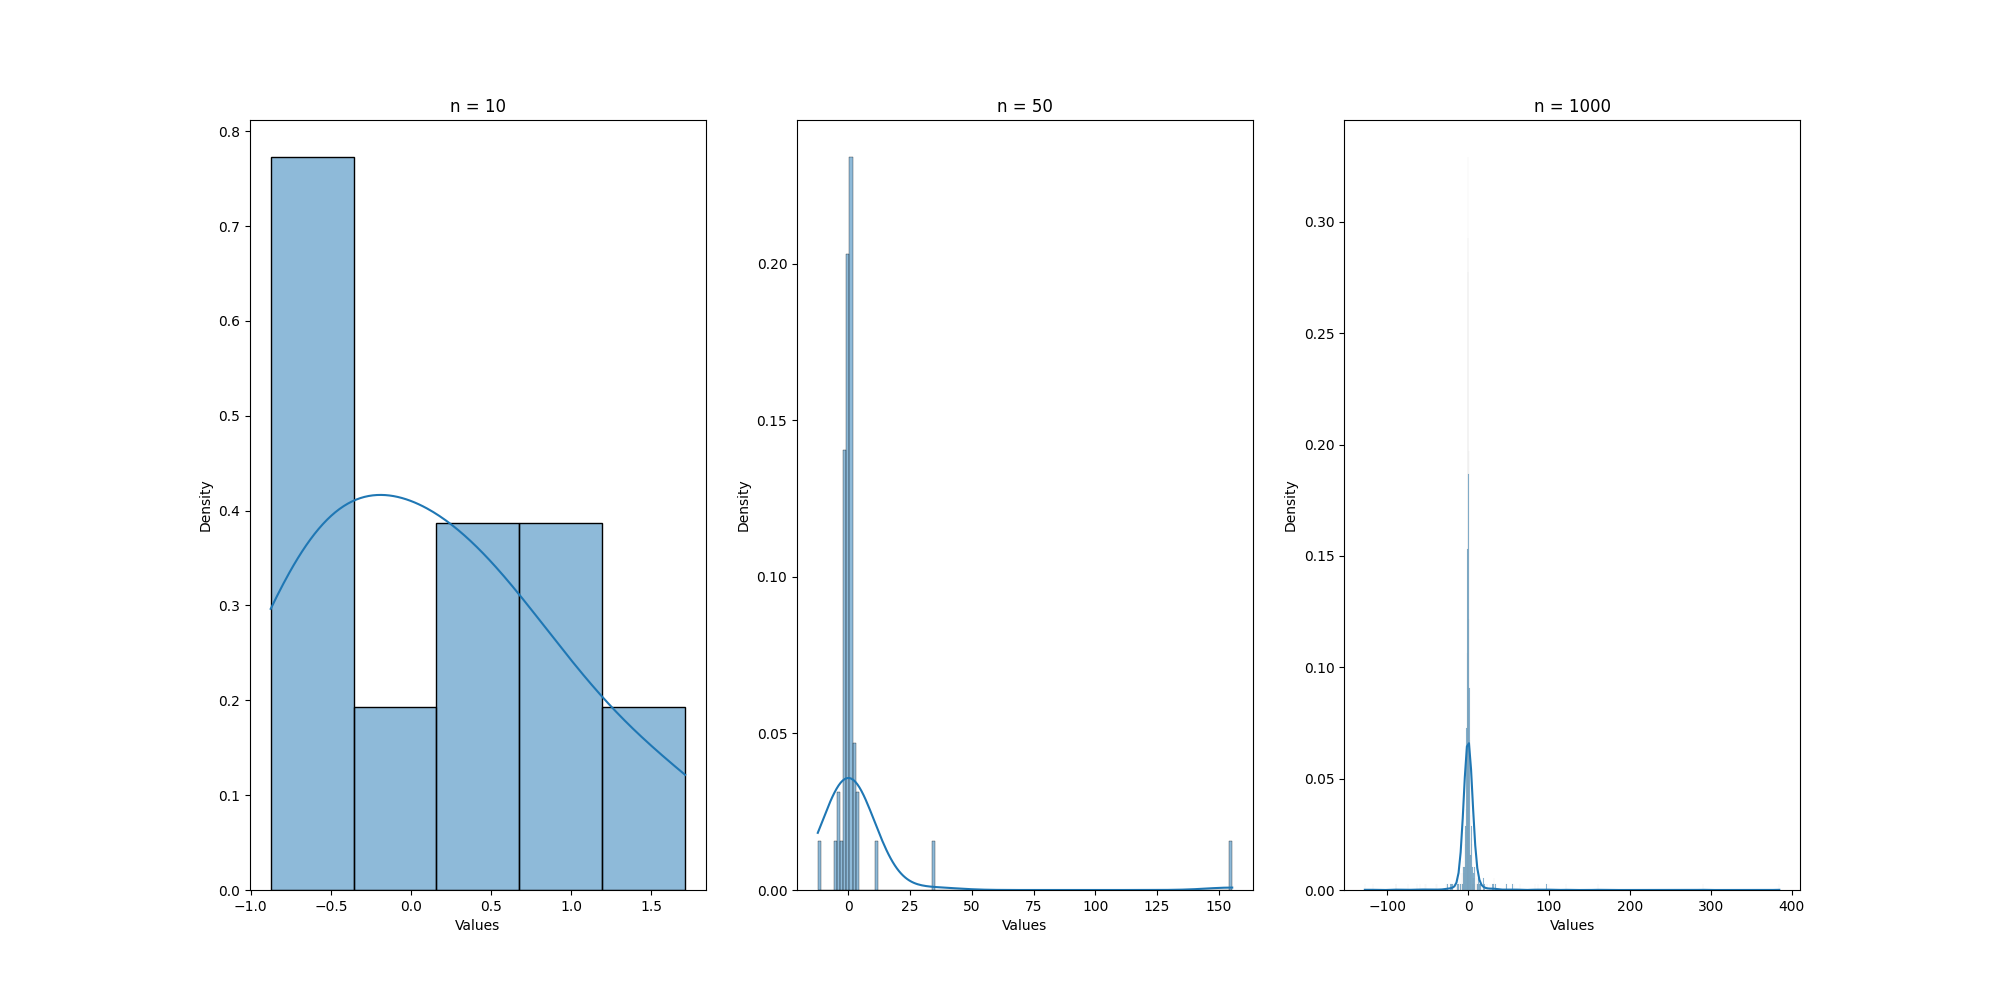
\includegraphics[width = 1.12\linewidth]{graphics/lab1_cauchy.png}
			\caption{Распределение Коши \ \eqref{eq:cauchy}}
		\end{center}
	\end{figure}

	\newpage

	\begin{figure}[htbp!]
		\begin{center}
			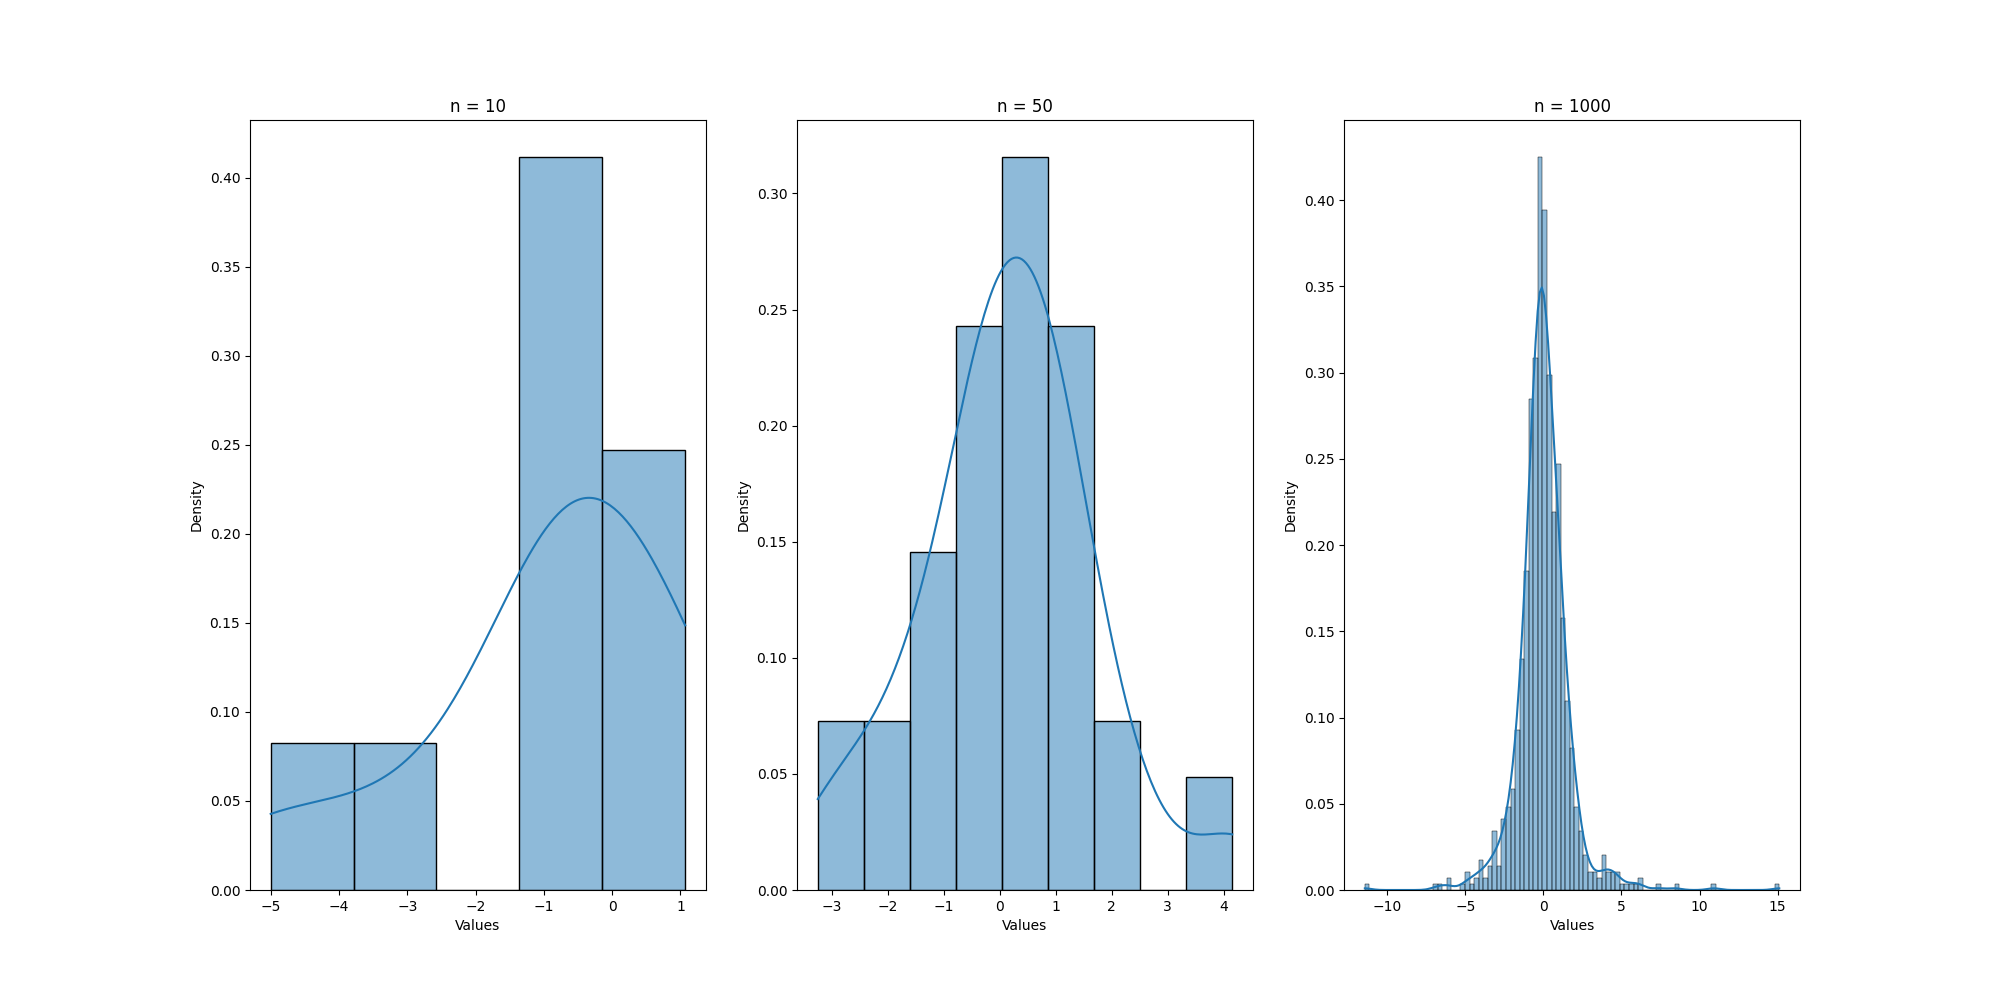
\includegraphics[width = 1.12\linewidth]{graphics/lab1_student.png}
			\caption{Распределение Стьюдента \ \eqref{eq:student}}
		\end{center}
	\end{figure}

	\begin{figure}[htbp!]
		\begin{center}
			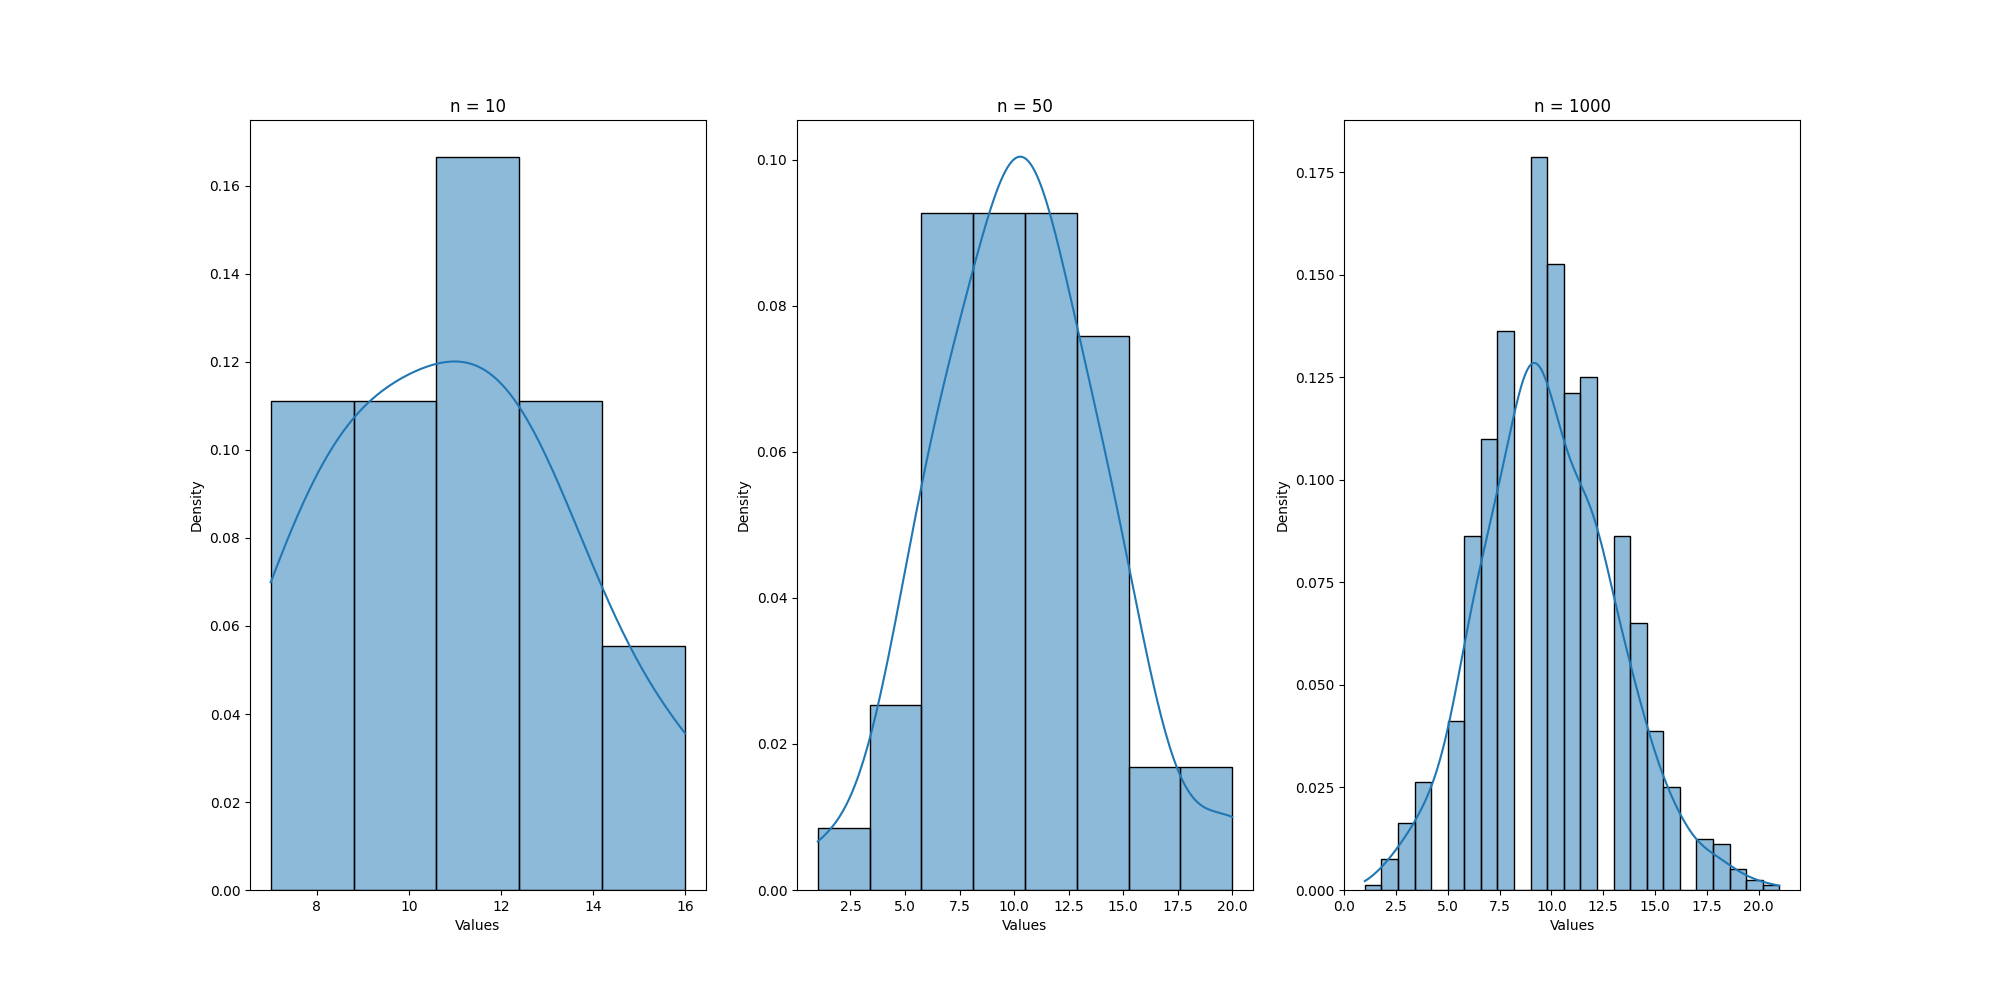
\includegraphics[width = 1.12\linewidth]{graphics/lab1_poisson.png}
			\caption{Распределение Пуассона \ \eqref{eq:poisson}}
		\end{center}
	\end{figure}

	\begin{figure}[htbp!]
		\begin{center}
			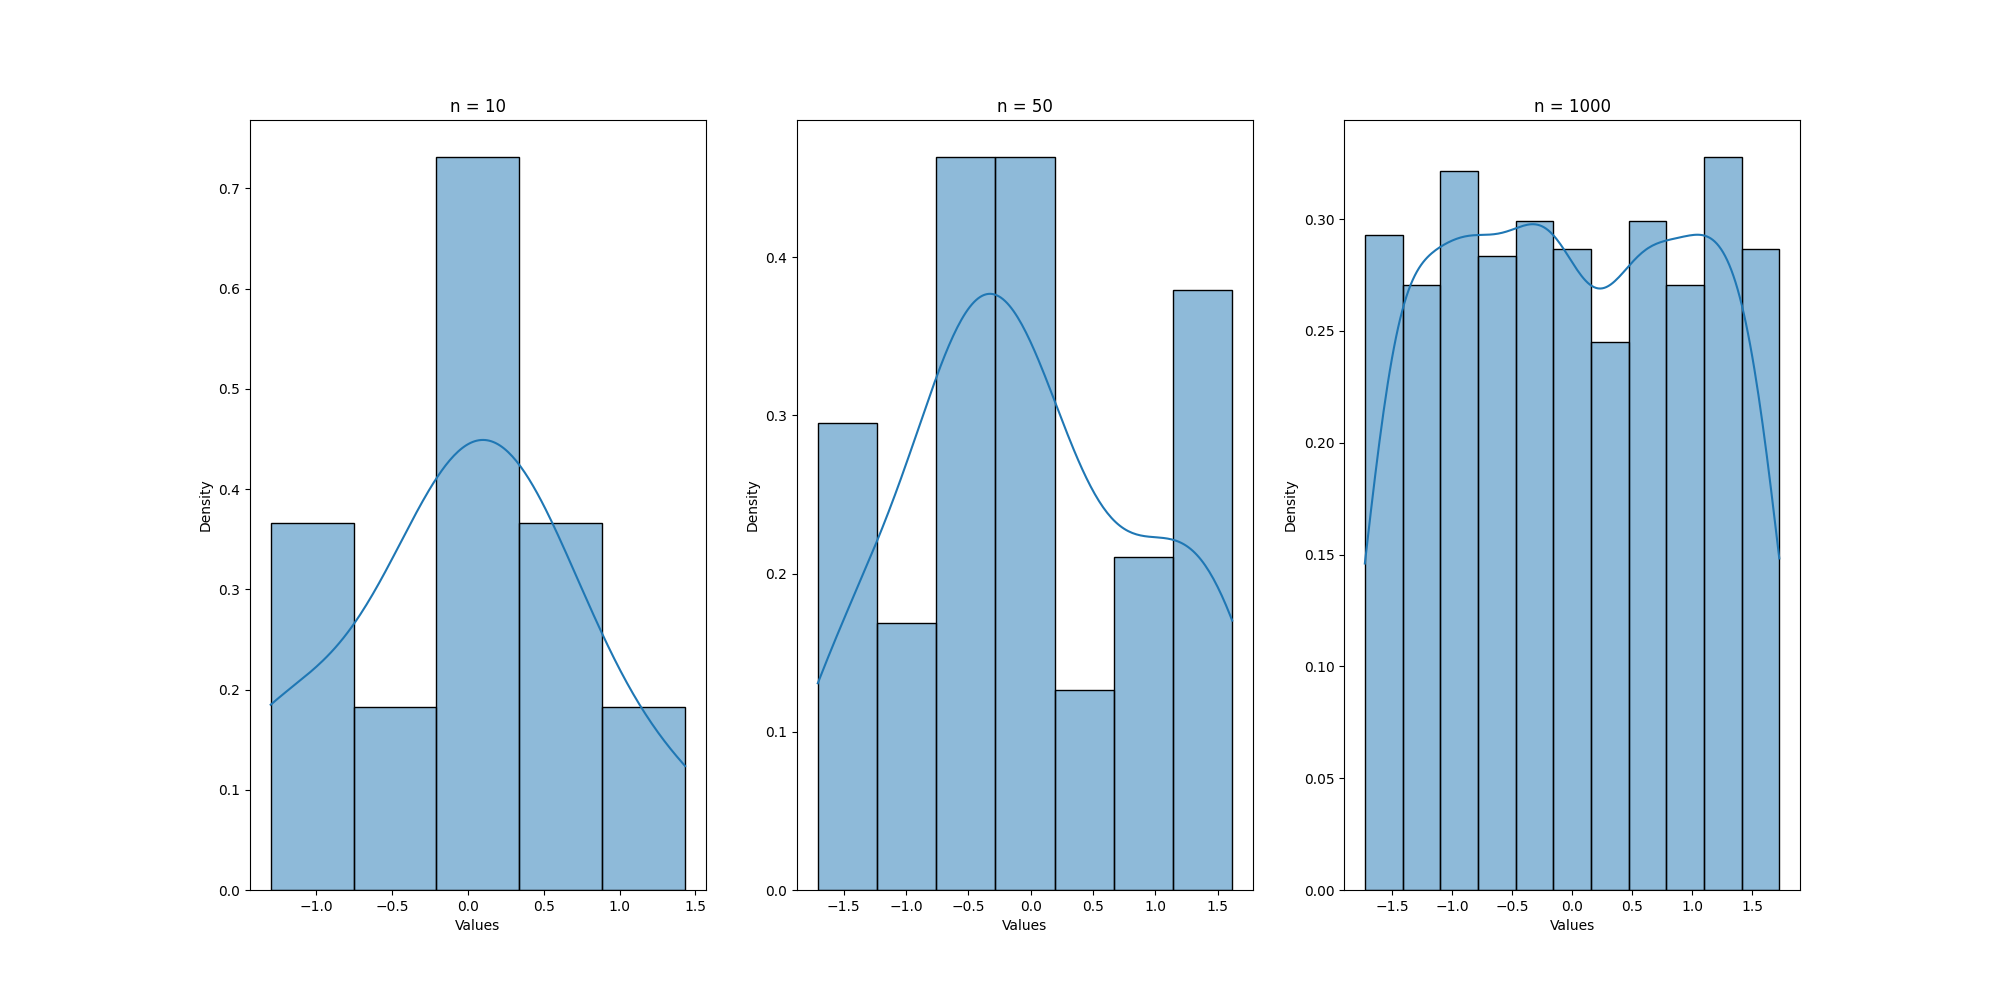
\includegraphics[width = 1.12\linewidth]{graphics/lab1_uniform.png}
			\caption{Равномерное распределение \ \eqref{eq:uniform}}
		\end{center}
	\end{figure}

	\newpage

	\subsection{Характеристики положения и рассеяния}

	\begin{table}[htbp!]
		\centering
		\begin{tabular}{ |c|c|c|c|c|c| }
			\hline
			n = 10 & & & & & \\
			\hline
			&\( \overline{x}\ \eqref{eq:mean} \) & \( med\ x \ \eqref{eq:median} \) & \( z_{R} \ \eqref{eq:half_sum_of_extremal_elements} \) & \( z_{Q} \ \eqref{eq:half_sum_of_quartiles} \) & \( z_{tr} \ \eqref{eq:trimmed_mean} \)\\
			\hline
			\( E(z) \ \eqref{eq:expected_value} \) & \( -1.747 \times 10^{-2} \) & \( -1.928 \times 10^{-2} \) & \( -1.949 \times 10^{-2} \) & \( -1.449 \times 10^{-2} \) & \( -7.937 \times 10^{-3} \) \\
			\hline
			\( D(z) \ \eqref{eq:dispersion}  \) & \( 1.009 \times 10^{-1} \) & \( 1.427 \times 10^{-1} \) & \( 1.878 \times 10^{-1} \) & \( 1.154 \times 10^{-1} \) & \( 1.608 \times 10^{-1} \) \\
			\hline
			n = 50 & & & & & \\
			\hline
			&\( \overline{x}\ \eqref{eq:mean} \) & \( med\ x \ \eqref{eq:median} \) & \( z_{R} \ \eqref{eq:half_sum_of_extremal_elements} \) & \( z_{Q} \ \eqref{eq:half_sum_of_quartiles} \) & \( z_{tr} \ \eqref{eq:trimmed_mean} \)\\
			\hline
			\( E(z) \ \eqref{eq:expected_value} \) & \( -7.937 \times 10^{-3} \) & \( 1.009 \times 10^{-1} \) & \( 1.427 \times 10^{-1} \) & \( 1.878 \times 10^{-1} \) & \( 1.154 \times 10^{-1} \) \\
			\hline
			\( D(z) \ \eqref{eq:dispersion} \) & \( 9.941 \times 10^{-3}  \) & \( 1.554 \times 10^{-2} \) & \( 9.559 \times 10^{-2} \) & \( 1.239 \times 10^{-2} \) & \( 2.000 \times 10^{-2} \) \\
			\hline
			n = 1000 & & & & & \\
			\hline
			&\( \overline{x}\ \eqref{eq:mean} \) & \( med\ x \ \eqref{eq:median} \) & \( z_{R} \ \eqref{eq:half_sum_of_extremal_elements} \) & \( z_{Q} \ \eqref{eq:half_sum_of_quartiles} \) & \( z_{tr} \ \eqref{eq:trimmed_mean} \)\\
			\hline
			\( E(z) \ \eqref{eq:expected_value} \) & \( 3.800 \times 10^{-5} \) & \( -1.779 \times 10^{-3} \) & \( -2.971 \times 10^{-3} \) & \( 1.002 \times 10^{-3} \) & \( -8.500 \times 10^{-5} \) \\
			\hline
			\( D(z) \ \eqref{eq:dispersion} \) & \( 9.850 \times 10^{-4} \) & \( 1.682 \times 10^{-3} \) & \( 6.138 \times 10^{-2} \) & \( 1.243 \times 10^{-3} \) & \( 1.939 \times 10^{-3} \) \\
			\hline
		\end{tabular}
		\caption{Нормальное распределение}
	\end{table}

	\begin{table}[htbp!]
		\centering
		\begin{tabular}{ |c|c|c|c|c|c| }
			\hline
			n = 10 & & & & & \\
			\hline
			&\( \overline{x}\ \eqref{eq:mean} \) & \( med\ x \ \eqref{eq:median} \) & \( z_{R} \ \eqref{eq:half_sum_of_extremal_elements} \) & \( z_{Q} \ \eqref{eq:half_sum_of_quartiles} \) & \( z_{tr} \ \eqref{eq:trimmed_mean} \)\\
			\hline
			\( E(z) \ \eqref{eq:expected_value} \) & \( -4.724 \) & \( -1.599 \times 10^{-2} \) & \( -2.361 \times 10 \) & \( -1.518 \times 10^{-2} \) & \( -8.311 \) \\
			\hline
			\( D(z) \ \eqref{eq:dispersion}  \) & \( 1.148 \times 10^{4} \) & \( 3.371 \times 10^{-1} \) & \( 2.865 \times 10^{5} \) & \( 1.164 \) & \( 3.170 \times 10^{4} \) \\
			\hline
			n = 50 & & & & & \\
			\hline
			&\( \overline{x}\ \eqref{eq:mean} \) & \( med\ x \ \eqref{eq:median} \) & \( z_{R} \ \eqref{eq:half_sum_of_extremal_elements} \) & \( z_{Q} \ \eqref{eq:half_sum_of_quartiles} \) & \( z_{tr} \ \eqref{eq:trimmed_mean} \)\\
			\hline
			\( E(z) \ \eqref{eq:expected_value} \) & \( 7.817 \times 10^{-1} \) & \( 1.222 \times 10^{-2} \) & \( 3,703 \times 10 \) & \( 8.637 \times 10^{-3} \) & \( 8.573 \times 10^{-1} \) \\
			\hline
			\( D(z) \ \eqref{eq:dispersion} \) & \( 4.319 \times 10^2 \) & \( 2.532 \times 10^{-2} \) & \( 1.060 \times 10^6 \) & \( 5.501 \times 10^{-2} \) & \( 1.677 \times 10^2 \) \\
			\hline
			n = 1000 & & & & & \\
			\hline
			&\( \overline{x}\ \eqref{eq:mean} \) & \( med\ x \ \eqref{eq:median} \) & \( z_{R} \ \eqref{eq:half_sum_of_extremal_elements} \) & \( z_{Q} \ \eqref{eq:half_sum_of_quartiles} \) & \( z_{tr} \ \eqref{eq:trimmed_mean} \)\\
			\hline
			\( E(z) \ \eqref{eq:expected_value} \) & \( -3.361 \times 10^{-1} \) & \( -1.532 \times 10^{-3} \) & \( -1.290 \times 10^2 \) & \( -1.540 \times 10^{-3} \) & \( -4.972 \times 10^{-2} \) \\
			\hline
			\( D(z) \ \eqref{eq:dispersion} \) & \( 2.406 \times 10^2 \) & \( 2.310 \times 10^{-3} \) & \( 5.036 \times 10^7 \) & \( 4.735 \times 10^{-3} \) & \( 1.743 \times 10^2 \) \\
			\hline
		\end{tabular}
		\caption{Распределение Коши}
	\end{table}

	\begin{table}[htbp!]
		\centering
		\begin{tabular}{ |c|c|c|c|c|c| }
			\hline
			n = 10 & & & & & \\
			\hline
			&\( \overline{x}\ \eqref{eq:mean} \) & \( med\ x \ \eqref{eq:median} \) & \( z_{R} \ \eqref{eq:half_sum_of_extremal_elements} \) & \( z_{Q} \ \eqref{eq:half_sum_of_quartiles} \) & \( z_{tr} \ \eqref{eq:trimmed_mean} \)\\
			\hline
			\( E(z) \ \eqref{eq:expected_value} \) & \( 1.626 \times 10^{-2} \) & \( 4.667 \times 10^{-3} \) & \( 4.092 \times 10^{-2} \) & \( 1.432 \times 10^{-2} \) & \( 7.500 \times 10^{-4} \) \\
			\hline
			\( D(z) \ \eqref{eq:dispersion}  \) & \( 2.591 \times 10^{-1} \) & \( 1.838 \times 10^{-1} \) & \( 1.659 \) & \( 1.846 \times 10^{-1} \) & \( 4.319 \times 10^{-1} \) \\
			\hline
			n = 50 & & & & & \\
			\hline
			&\( \overline{x}\ \eqref{eq:mean} \) & \( med\ x \ \eqref{eq:median} \) & \( z_{R} \ \eqref{eq:half_sum_of_extremal_elements} \) & \( z_{Q} \ \eqref{eq:half_sum_of_quartiles} \) & \( z_{tr} \ \eqref{eq:trimmed_mean} \)\\
			\hline
			\( E(z) \ \eqref{eq:expected_value} \) & \( -2.158 \times 10^{-3} \) & \( -1.389 \times 10^{-3} \) & \( 2.124 \times 10^{-2} \) & \( 3.592 \times 10^{-3} \) & \( -1.675 \times 10^{-2} \) \\
			\hline
			\( D(z) \ \eqref{eq:dispersion} \) & \( 2.691 \times 10^{-2} \) & \( 1.905 \times 10^{-2} \) & \( 9.894 \) & \( 1.848 \times 10^{-2} \) & \( 5.278 \times 10^{-2} \) \\
			\hline
			n = 1000 & & & & & \\
			\hline
			&\( \overline{x}\ \eqref{eq:mean} \) & \( med\ x \ \eqref{eq:median} \) & \( z_{R} \ \eqref{eq:half_sum_of_extremal_elements} \) & \( z_{Q} \ \eqref{eq:half_sum_of_quartiles} \) & \( z_{tr} \ \eqref{eq:trimmed_mean} \)\\
			\hline
			\( E(z) \ \eqref{eq:expected_value} \) & \( 3.350 \times 10^{-4} \) & \( -2.380 \times 10^{-4} \) & \( -5.482 \times 10^{-2} \) & \( 1.620 \times 10^{-4} \) & \( 6.790 \times 10^{-4} \) \\
			\hline
			\( D(z) \ \eqref{eq:dispersion} \) & \( 2.898 \times 10^{-3} \) & \( 1.903 \times 10^{-3} \) & \( 3.253 \times 10 \) & \( 1.944 \times 10^{-3} \) & \( 5.656 \times 10^{-3} \) \\
			\hline
		\end{tabular}
		\caption{Распределение Стьюдента}
	\end{table}

	\begin{table}[htbp!]
		\centering
		\begin{tabular}{ |c|c|c|c|c|c| }
			\hline
			n = 10 & & & & & \\
			\hline
			&\( \overline{x}\ \eqref{eq:mean} \) & \( med\ x \ \eqref{eq:median} \) & \( z_{R} \ \eqref{eq:half_sum_of_extremal_elements} \) & \( z_{Q} \ \eqref{eq:half_sum_of_quartiles} \) & \( z_{tr} \ \eqref{eq:trimmed_mean} \)\\
			\hline
			\( E(z) \ \eqref{eq:expected_value} \) & \( 1.000 \times 10 \) & \( 9.874 \) & \( 1.029 \times 10 \) & \( 9.918 \) & \( 9.937 \) \\
			\hline
			\( D(z) \ \eqref{eq:dispersion}  \) & \( 1.082 \) & \( 1.478 \) & \( 2.018 \) & \( 1.284 \) & \( 1.699 \) \\
			\hline
			n = 50 & & & & & \\
			\hline
			&\( \overline{x}\ \eqref{eq:mean} \) & \( med\ x \ \eqref{eq:median} \) & \( z_{R} \ \eqref{eq:half_sum_of_extremal_elements} \) & \( z_{Q} \ \eqref{eq:half_sum_of_quartiles} \) & \( z_{tr} \ \eqref{eq:trimmed_mean} \)\\
			\hline
			\( E(z) \ \eqref{eq:expected_value} \) & \( 1.001 \times 10 \) & \( 9.856 \) & \( 1.090 \times 10 \) & \( 9.945 \) & \( 1.001 \times 10 \) \\
			\hline
			\( D(z) \ \eqref{eq:dispersion} \) & \( 9.575 \times 10^{-2} \) & \( 1.974 \times 10^{-1} \) & \( 9.572 \times 10^{-1} \) & \( 1.398 \times 10^{-1} \) & \( 2.048 \times 10^{-1} \) \\
			\hline
			n = 1000 & & & & & \\
			\hline
			&\( \overline{x}\ \eqref{eq:mean} \) & \( med\ x \ \eqref{eq:median} \) & \( z_{R} \ \eqref{eq:half_sum_of_extremal_elements} \) & \( z_{Q} \ \eqref{eq:half_sum_of_quartiles} \) & \( z_{tr} \ \eqref{eq:trimmed_mean} \)\\
			\hline
			\( E(z) \ \eqref{eq:expected_value} \) & \( 1.000 \times 10 \) & \( 9.997 \) & \( 1.163 \times 10 \) & \( 9.994 \) & \( 1.000 \times 10 \) \\
			\hline
			\( D(z) \ \eqref{eq:dispersion} \) & \( 1.014 \times 10^{-2} \) & \( 2.991 \times 10^{-3} \) & \( 6.344 \times 10^{-1} \) & \( 2.964 \times 10^{-3} \) & \( 2.072 \times 10^{-2} \) \\
			\hline
		\end{tabular}
		\caption{Распределение Пуассона}
	\end{table}

	\begin{table}[htbp!]
		\centering
		\begin{tabular}{ |c|c|c|c|c|c| }
			\hline
			n = 10 & & & & & \\
			\hline
			&\( \overline{x}\ \eqref{eq:mean} \) & \( med\ x \ \eqref{eq:median} \) & \( z_{R} \ \eqref{eq:half_sum_of_extremal_elements} \) & \( z_{Q} \ \eqref{eq:half_sum_of_quartiles} \) & \( z_{tr} \ \eqref{eq:trimmed_mean} \)\\
			\hline
			\( E(z) \ \eqref{eq:expected_value} \) & \( -5.450 \times 10^{-3} \) & \( -6.939 \times 10^{-3} \) & \( -5.412 \times 10^{-3} \) & \( -7.901 \times 10^{-3} \) & \( -1.561 \times 10^{-2} \) \\
			\hline
			\( D(z) \ \eqref{eq:dispersion}  \) & \( 1.041 \times 10^{-1} \) & \( 2.402 \times 10^{-1} \) & \( 4.402 \times 10^{-2} \) & \( 1.443 \times 10^{-1} \) & \( 1.722 \times 10^{-1} \) \\
			\hline
			n = 50 & & & & & \\
			\hline
			&\( \overline{x}\ \eqref{eq:mean} \) & \( med\ x \ \eqref{eq:median} \) & \( z_{R} \ \eqref{eq:half_sum_of_extremal_elements} \) & \( z_{Q} \ \eqref{eq:half_sum_of_quartiles} \) & \( z_{tr} \ \eqref{eq:trimmed_mean} \)\\
			\hline
			\( E(z) \ \eqref{eq:expected_value} \) & \( -1.915 \times 10^{-3} \) & \( -6.312 \times 10^{-3} \) & \( -1.349 \times 10^{-3} \) & \( 1.960 \times 10^{-3} \) & \( -4.766 \times 10^{-3} \) \\
			\hline
			\( D(z) \ \eqref{eq:dispersion} \) & \( 1.002 \times 10^{-2} \) & \( 2.972 \times 10^{-2} \) & \( 5.990 \times 10^{-4} \) & \( 1.428 \times 10^{-2} \) & \( 1.894 \times 10^{-2} \) \\
			\hline
			n = 1000 & & & & & \\
			\hline
			&\( \overline{x}\ \eqref{eq:mean} \) & \( med\ x \ \eqref{eq:median} \) & \( z_{R} \ \eqref{eq:half_sum_of_extremal_elements} \) & \( z_{Q} \ \eqref{eq:half_sum_of_quartiles} \) & \( z_{tr} \ \eqref{eq:trimmed_mean} \)\\
			\hline
			\( E(z) \ \eqref{eq:expected_value} \) & \( 4.700 \times 10^{-4} \) & \( 9.240 \times 10^{-4} \) & \( -1.330 \times 10^{-4} \) & \( -3.550 \times 10^{-4} \) & \( -3.870 \times 10^{-4} \) \\
			\hline
			\( D(z) \ \eqref{eq:dispersion} \) & \( 1.014 \times 10^{-3} \) & \( 3.127 \times 10^{-3} \) & \( 5.000 \times 10^{-6} \) & \( 1.469 \times 10^{-3} \) & \( 1.887 \times 10^{-3} \) \\
			\hline
		\end{tabular}
		\caption{Равномерное распределение}
	\end{table}

	\newpage

	\section{Выводы}

	В процессе выполнения лабораторной работы был проведен анализ пяти уникальных распределений: нормальное, Коши, Стьюдента, Пуассона и равномерное.
	Были сгенерированы выборки разных объемов для каждого из них - 10, 50 и 1000 элементов.
	Были созданы гистограммы каждого распределения и нанесены на них графики плотности соответствующих распределений, что облегчило наглядное сопоставление формы распределения выборок с их теоретическими аналогами.
	Были также рассчитаны разные показатели положения и рассеяния для каждой выборки, включая выборочную среднюю величину, медиану, полусумму крайних элементов выборки, полусумму квартилей и усеченное среднее.
	Использовалась стандартная формула для оценки дисперсии. \\

	На основании полученных данных были сделаны следующие выводы:

	\begin{enumerate}
		\item В случае нормального распределения, оценки показателей положения и рассеяния становятся ближе к их теоретическим значениям по мере увеличения размера выборки.
		\item Для распределения Коши показатели положения и рассеяния менее стабильны и могут сильно отличаться от теоретических даже при больших размерах выборки.
		\item Распределение Стьюдента при небольших размерах выборки также демонстрирует определенную нестабильность оценок, однако с увеличением размера выборки результаты становятся более точными.
		\item Для распределения Пуассона и равномерного распределения, оценки показателей положения и рассеяния кажутся стабильными при любом объеме выборки.
		\item В общем, выборочное среднее является наиболее чувствительным к экстремальным значениям по сравнению с медианой, особенно в меньших выборках. Однако с увеличением размера выборки, влияние этих экстремальных значений на среднее значение уменьшается. В то же время, медиана обычно более устойчива к выбросам и мало варьирует с изменением размера выборки.
		\item Медиана является чувствительной к типу распределения: в нормальном и распределении Стьюдента медиана равна среднему, в распределении Коши она дает надежные, устойчивые к выбросам оценки, в Пуассоновском приближается к среднему, и в равномерном равна половине суммы минимального и максимального значений.
	\end{enumerate}

	\section{Постановка задачи}

	\subsection{Боксплот Тьюки}

	Сгенерировать выборки размером 20 и 100 элементов. Построить для них боксплот Тьюки.

	\subsection{Доверительные интервалы для параметров нормального распределения}

	Сгенерировать выборки размером 20 и 100 элементов. Вычислить параметры положения и рассеяния:

	\begin{itemize}
		\item для нормального распределения,
		\item для произвольного распределения.
	\end{itemize}

	\section{Теоретическое обоснование}

	\subsection{Функции распределения}

	\begin{itemize}
		\item Нормальное распределение

		\begin{equation} \label{eq:normal}
			N(x, 0, 1) = \frac{1}{\sqrt{2\pi}}e^\frac{-x^2}{2}
		\end{equation}

		\item Распределение Коши

		\begin{equation} \label{eq:cauchy}
			C(x, 0, 1) = \frac{1}{\pi}\frac{1}{x^2+1}
		\end{equation}

		\item Распределение Стьюдента \( t(x, 0, 3) \) с тремя степенями свободы

		\begin{equation} \label{eq:student}
			t(x, 0, 3) = \frac{6\sqrt3}{\pi(3 + t^2)^2}
		\end{equation}

		\item Распределение Пуассона

		\begin{equation} \label{eq:poisson}
			P(k, 10) = \frac{10^k}{k!}e^{-10}
		\end{equation}

		\item Равномерное распределение

		\begin{equation} \label{eq:uniform}
			U(x, -\sqrt3, \sqrt3) = \begin{cases}
				\frac{1}{2\sqrt3}, & \; |x| \leq \sqrt3\\
				0, & \; |x| > \sqrt3
			\end{cases}
		\end{equation}
	\end{itemize}

	\subsection{Боксплот Тьюки}

	Боксплот (англ. box plot) — график, использующихся в описательной
	статистике, компактно изобрадающий одномерное распределение
	вероятностей. Такой вид диаграммы в удобной форме показывает медиану,
	нижний и верхний квартили и выбросы. Границами ящика служат первый и
	третий квартили, линия в середине ящика — медиана. Концы усов — края
	статистически значимой выборки (без выброса). Длину <<усов>> определяют
	разность первого квартиля и полутора межквартальных расстояний и сумма
	третьего квартиля и полутора межквартальных расстояний. Формула имеет
	вид

	\begin{equation} \label{eq:box_plot}
		X_1 = Q_1 - \frac{3}{2}(Q_3 - Q_1), \ X_2 = Q_3 + \frac{3}{2}(Q_3 - Q_1),
	\end{equation}

	где \( X_1 \) — нижняя граница уса, \( X_2 \) — верхняя граница уса,
	\( Q_1 \) — первый квартиль, \( Q_3 \) - третий квартиль. Данные,
	выходящие за границы усов (выбросы), отображаются на графике в виде
	маленьких кружков. Выбросами считаются величины \( х \), такие что:

	\begin{equation} \label{eq:outlier}
		\left[
			\begin{array}{ll}
					x < X_1^T \\
					x > X_2^T
			\end{array}
		\right .
	\end{equation}

	\subsection{Доверительные интервалы для параметров нормального
		распределения}

	Пусть \( F_T(x) \) — функция распределения Стьюдента с \( n - 1 \)
	степенями свободы. Полагаем, что \( 2F_T(x) - 1 = 1 - \alpha \), где
	\( \alpha \) — выбранный уровень значимости. Тогда
	\( F_T(x) = 1 - \alpha / 2 \). Пусть \( st_{1 - \alpha / 2}(n - 1) \) —
	квантиль распределения Стьюдента с \( n - 1 \) степенями свободы и
	порядка \( 1 - \alpha / 2 \). Тогда получаем

	\begin{equation} \label{eq:normal_mean_boundaries}
		P \left ( \overline x - \frac{st_{1 - \alpha / 2}(n - 1)}{\sqrt{n - 1}} < m
		< \overline x + \frac{st_{1 - \alpha / 2}(n - 1)}{\sqrt{n - 1}} \right ) =
		1 - \alpha,
	\end{equation}

	что и даст доверительный интервал для m с доверительной вероятностью
	\( \gamma = 1 \alpha \) для нормального распределения.

	Случайная величина \( n \frac{s^2}{\sigma^2} \) распределена по закону
	\( \chi^2 \) с \( n - 1 \) степенями свободы. Тогда

	\begin{equation} \label{eq:mean_boundaries}
		P \left ( \overline x - \frac{st_{1 - \alpha / 2}(n - 1)}{\sqrt{n - 1}} <
		m < \overline x + \frac{st_{1 - \alpha / 2}(n - 1)}{\sqrt{n - 1}} \right )
		= 1 - \alpha,
	\end{equation}

	\section{Описание работы}

	Лабораторные работы выполнены с использованием Python и его сторонних
	библиотек: \verb!numpy!, \verb!pandas!, \verb!matplotlib!, \verb!seaborn!.

	Ссылка на GitHub репозиторий:
	\href{https://github.com/vladimir-skvortsov/spbstu-mathematical-statistics}
	{https://github.com/vladimir-skvortsov/spbstu-mathematical-statistics}

	\newpage

	\section{Результаты}

	\subsection{Гистограммы и графики плотности распределения}

	\begin{figure}[htbp!]
		\begin{center}
			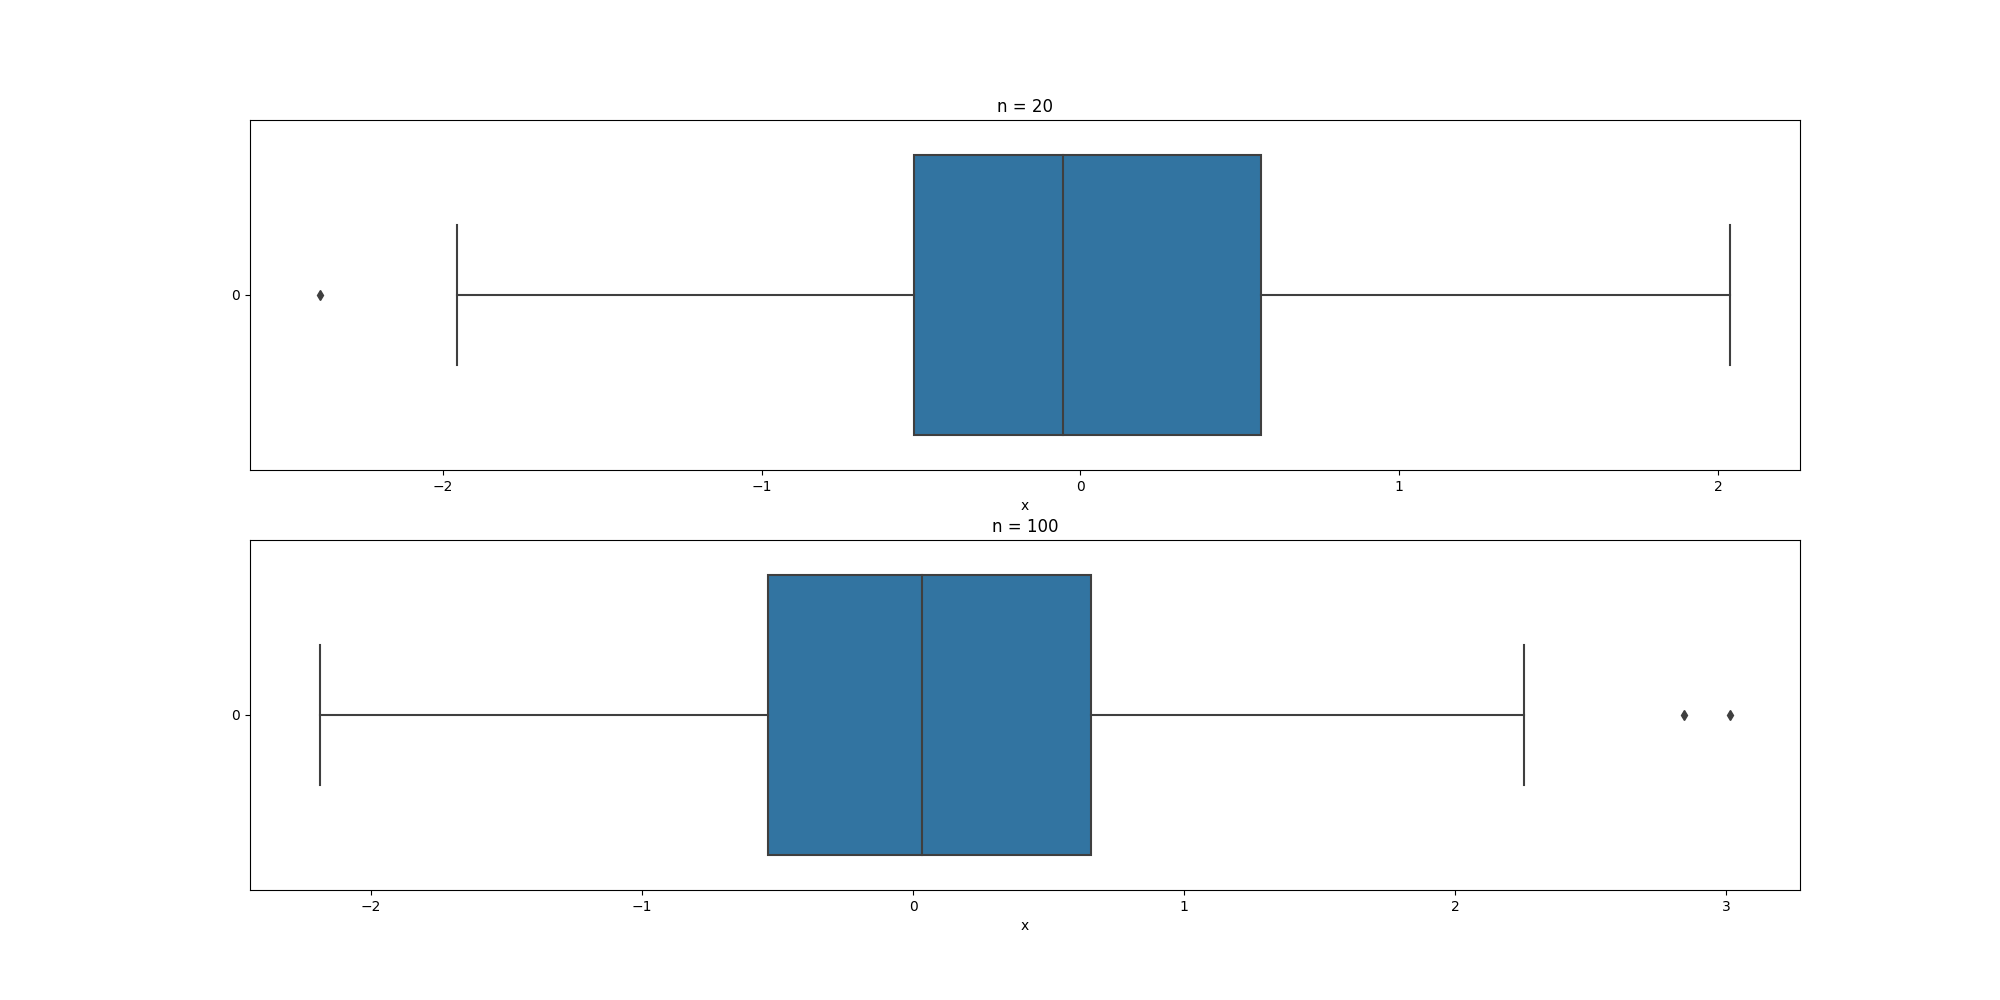
\includegraphics[width = 1.12\linewidth]{graphics/lab2_normal.png}
			\caption{Нормальное распределение \ \eqref{eq:normal}}
		\end{center}
	\end{figure}

	\begin{figure}[htbp!]
		\begin{center}
			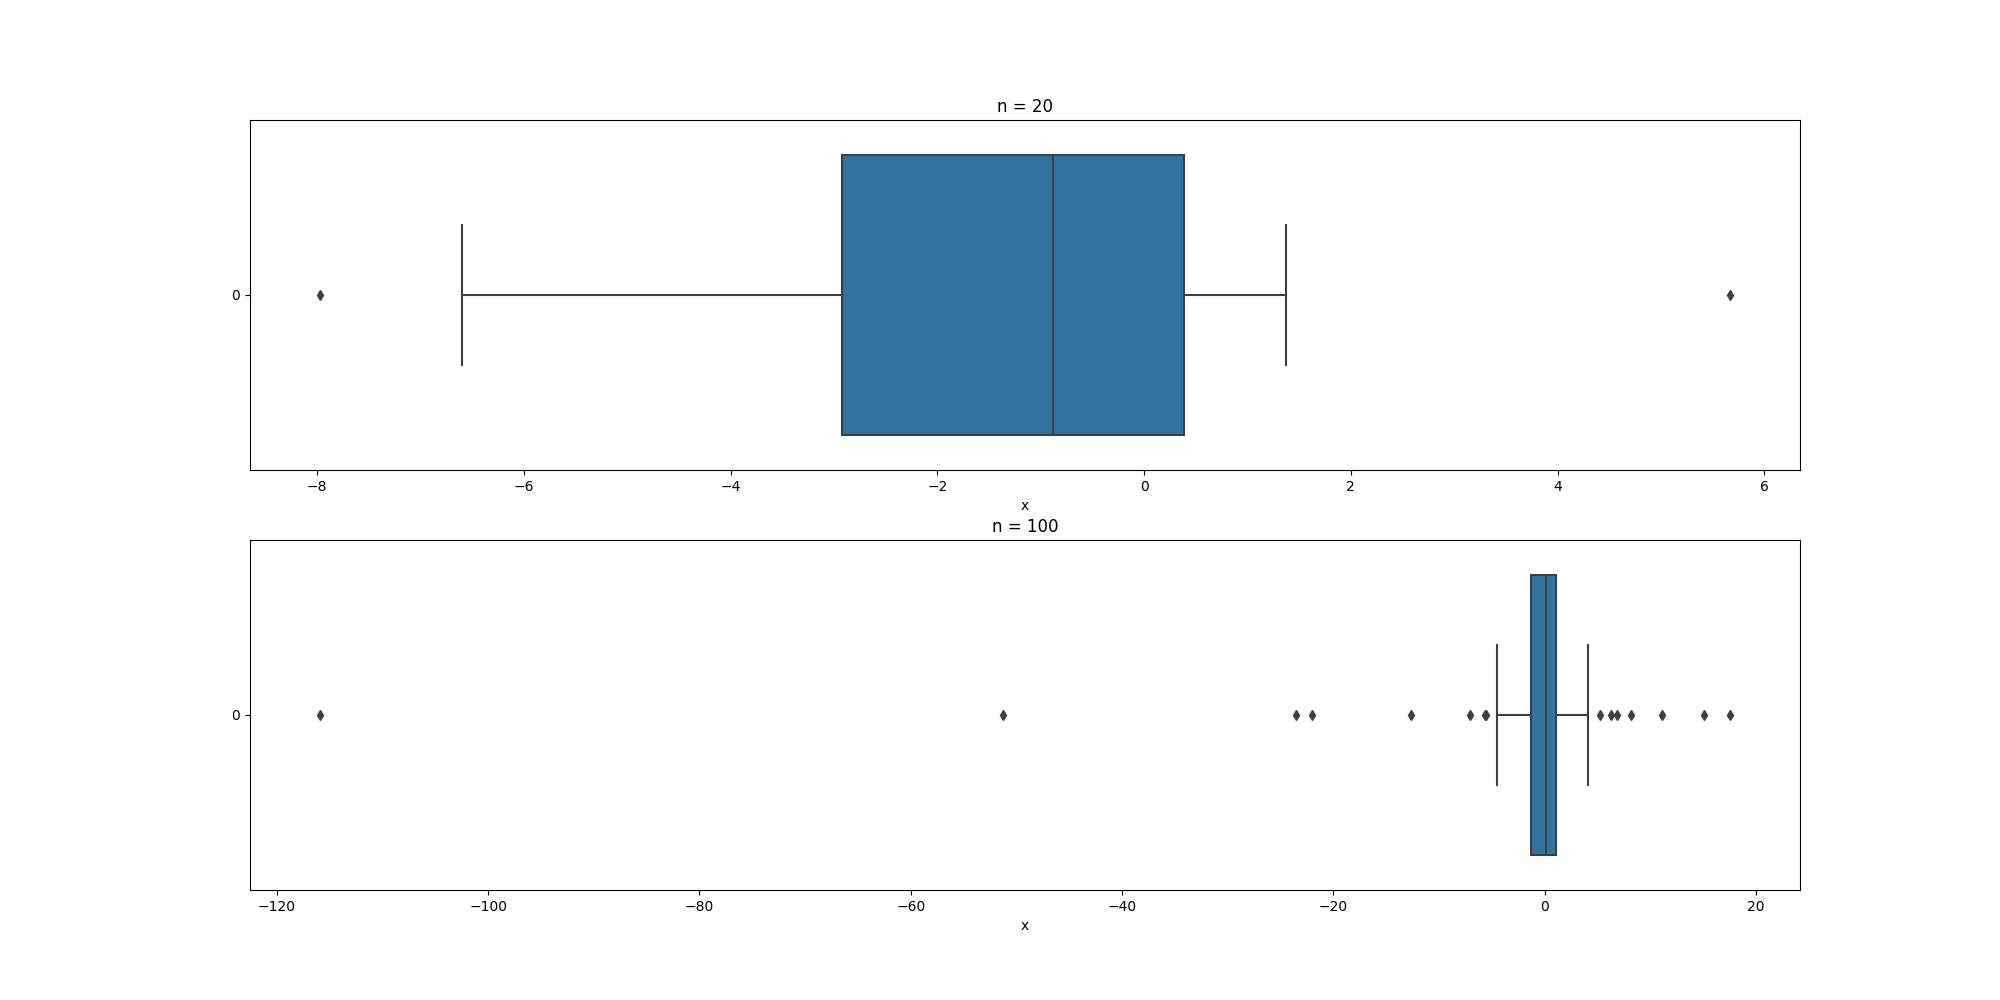
\includegraphics[width = 1.12\linewidth]{graphics/lab2_cauchy.png}
			\caption{Распределение Коши \ \eqref{eq:cauchy}}
		\end{center}
	\end{figure}

	\newpage

	\begin{figure}[htbp!]
		\begin{center}
			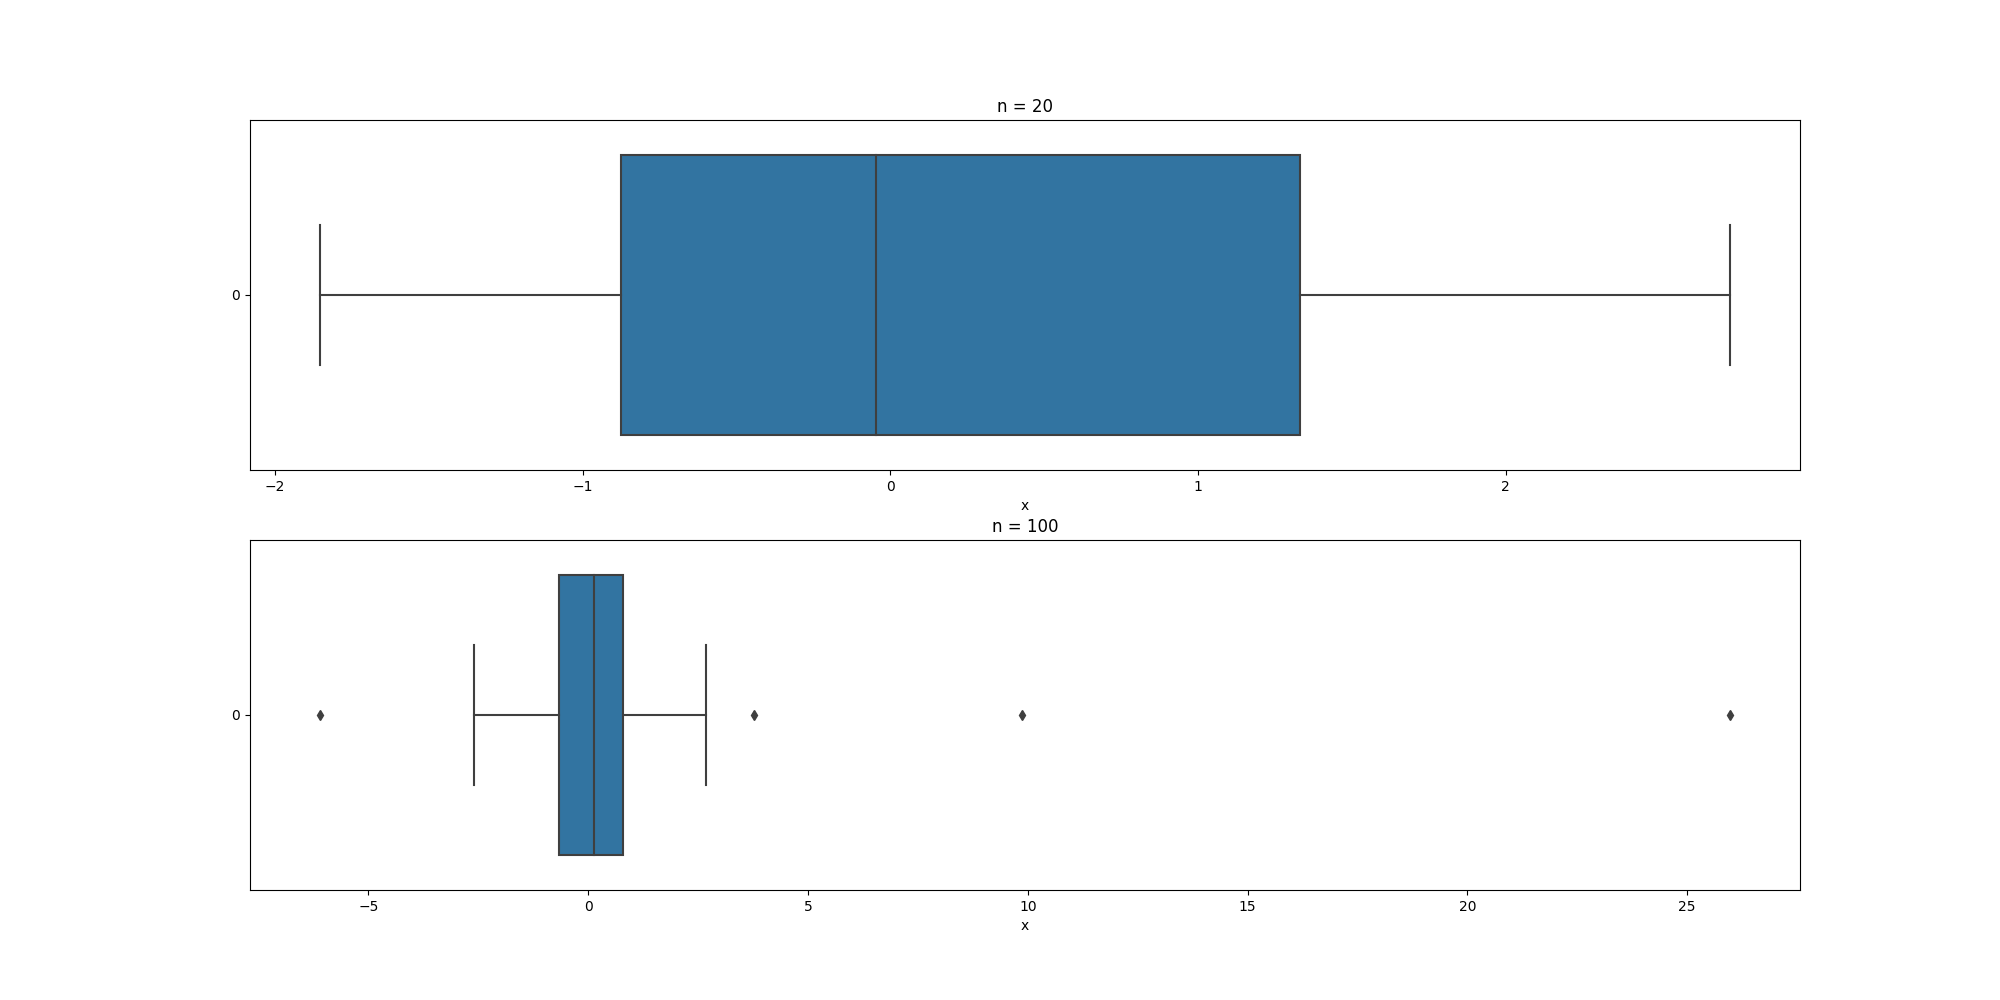
\includegraphics[width = 1.12\linewidth]{graphics/lab2_student.png}
			\caption{Распределение Стьюдента \ \eqref{eq:student}}
		\end{center}
	\end{figure}

	\begin{figure}[htbp!]
		\begin{center}
			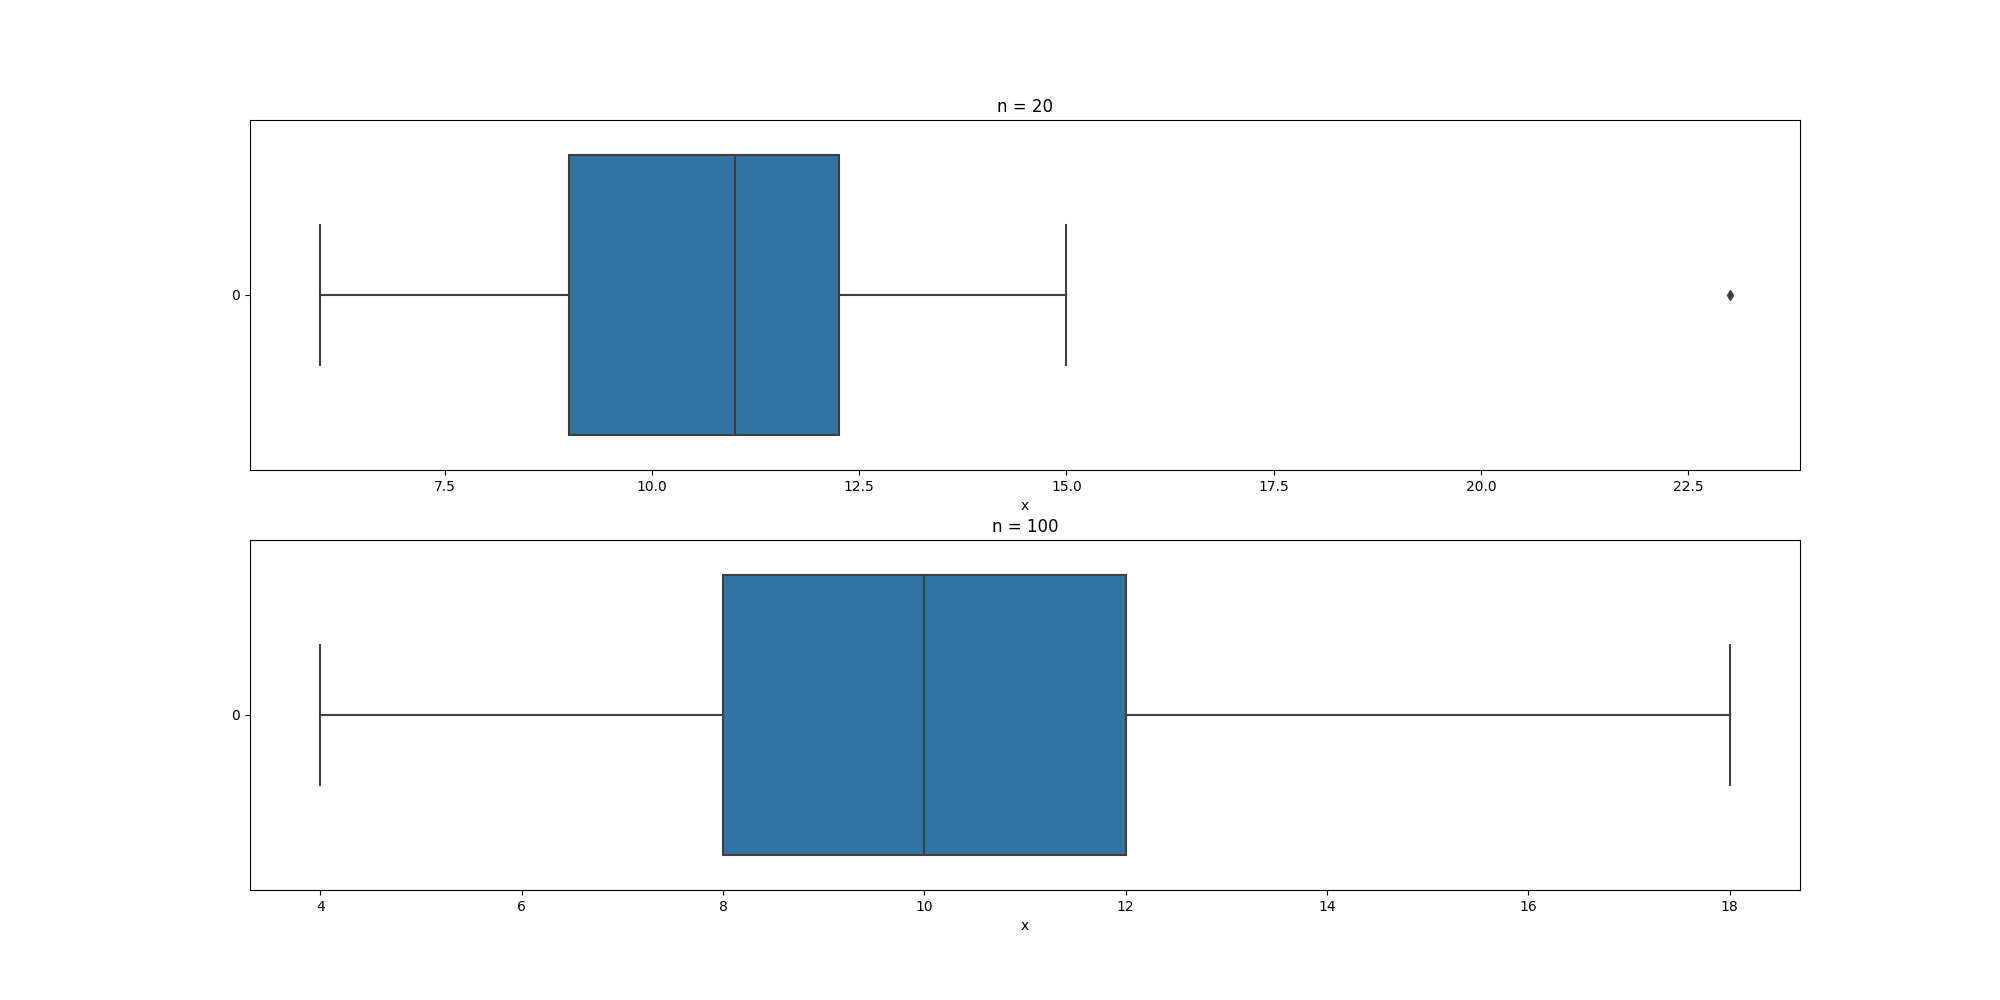
\includegraphics[width = 1.12\linewidth]{graphics/lab2_poisson.png}
			\caption{Распределение Пуассона \ \eqref{eq:poisson}}
		\end{center}
	\end{figure}

	\begin{figure}[htbp!]
		\begin{center}
			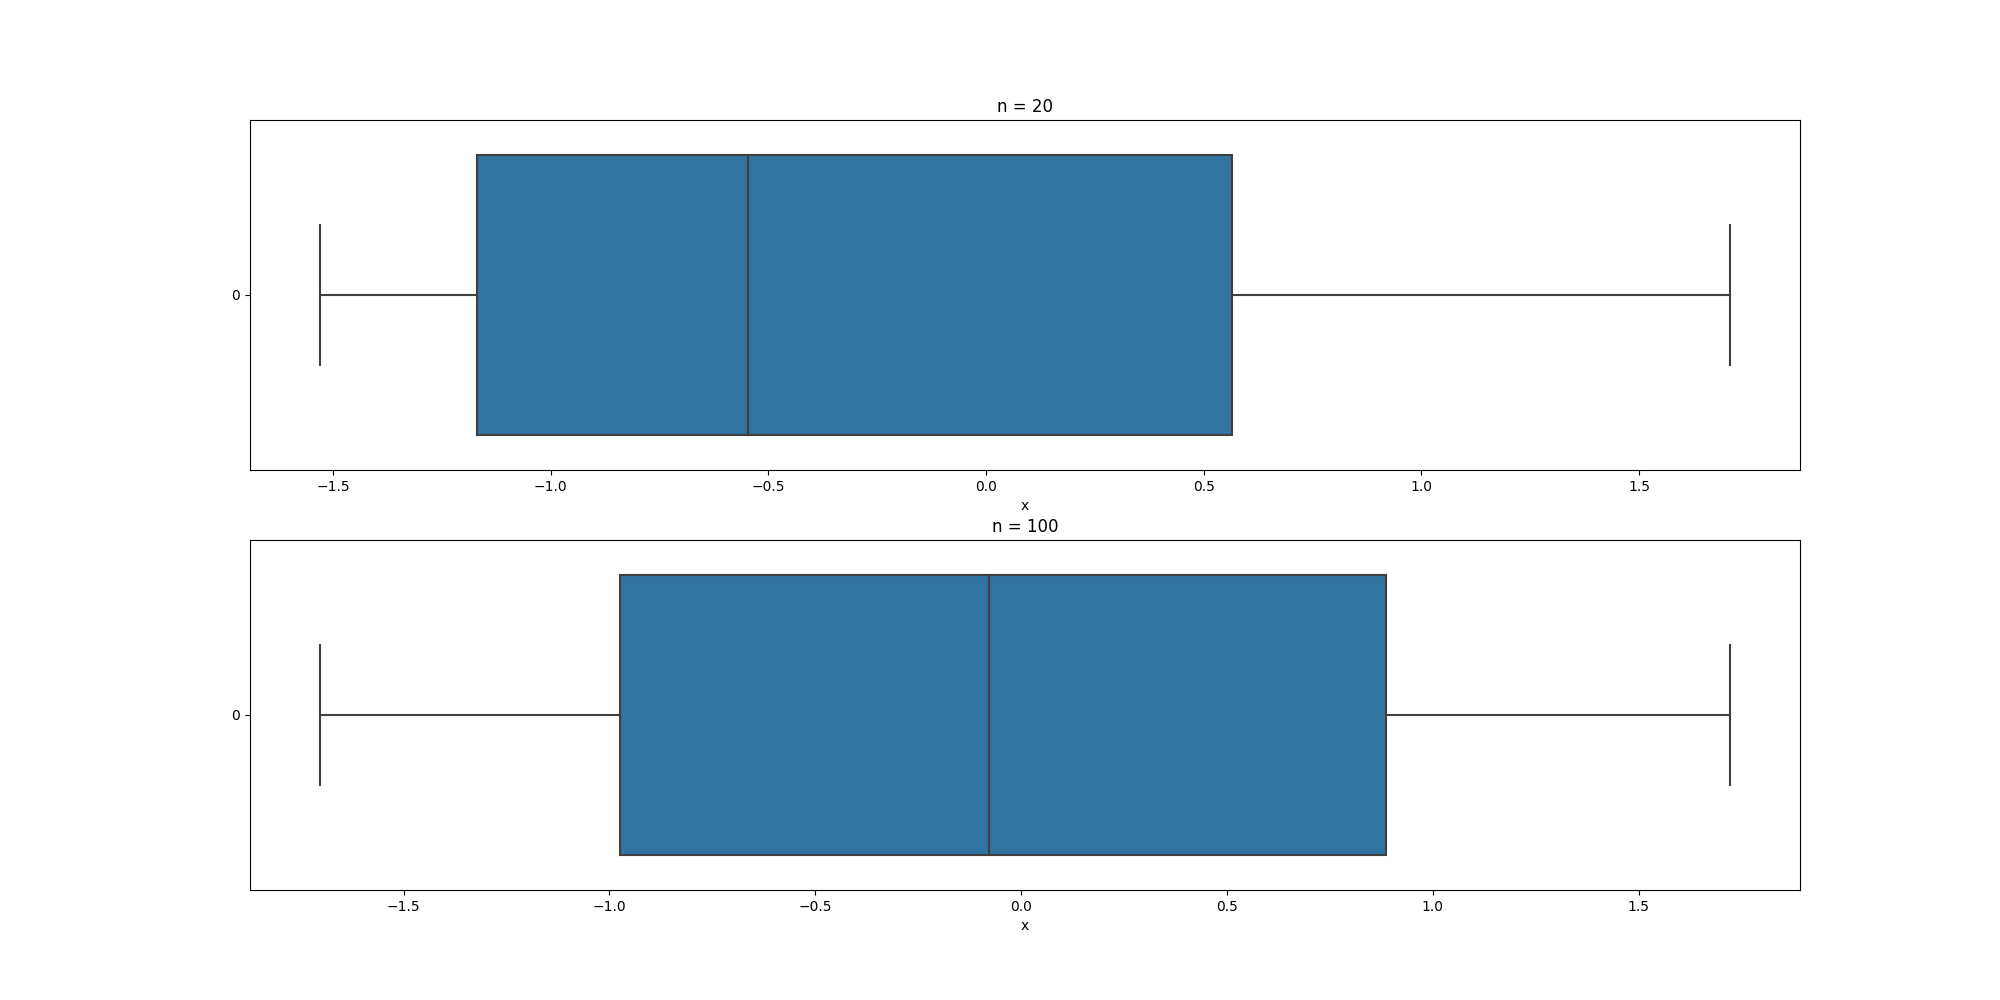
\includegraphics[width = 1.12\linewidth]{graphics/lab2_uniform.png}
			\caption{Равномерное распределение \ \eqref{eq:uniform}}
		\end{center}
	\end{figure}

	\newpage

	\subsection{Доверительные интервалы для параметров распределений}

	\begin{table}[htbp!]
		\centering
		\begin{tabular}{ |c|c|c| }
			\hline
			n = 20 & m & \( \sigma \) \\
			\hline
			& -0.43 < m < 0.37 & 0.66 < \( \sigma \) < 1.25 \\
			\hline
			n = 100 & m & \( \sigma \) \\
			\hline
			& -0.12 < m < 0.24 & 0.81 < \( \sigma \) < 1.07 \\
			\hline
		\end{tabular}
		\caption{Доверительные интервалы для параметров нормального
			распределения \eqref{eq:normal}}
	\end{table}

	\begin{table}[htbp!]
		\centering
		\begin{tabular}{ |c|c|c| }
			\hline
			n = 20 & \( m \) & \( \sigma \) \\
			\hline
			& 0.11 < \( m \) < 0.97 & 0.29 < \( \sigma \) < 0.33 \\
			\hline
			n = 100 & \( m \) & \( \sigma \) \\
			\hline
			& 0.30 < \( m \) < 0.67 & 0.28 < \( \sigma \) < 0.33 \\
			\hline
		\end{tabular}
		\caption{Доверительные интервалы для параметров произвольного
			распределения. Асимптотический подход}
	\end{table}

	\begin{figure}[htbp!]
		\begin{center}
			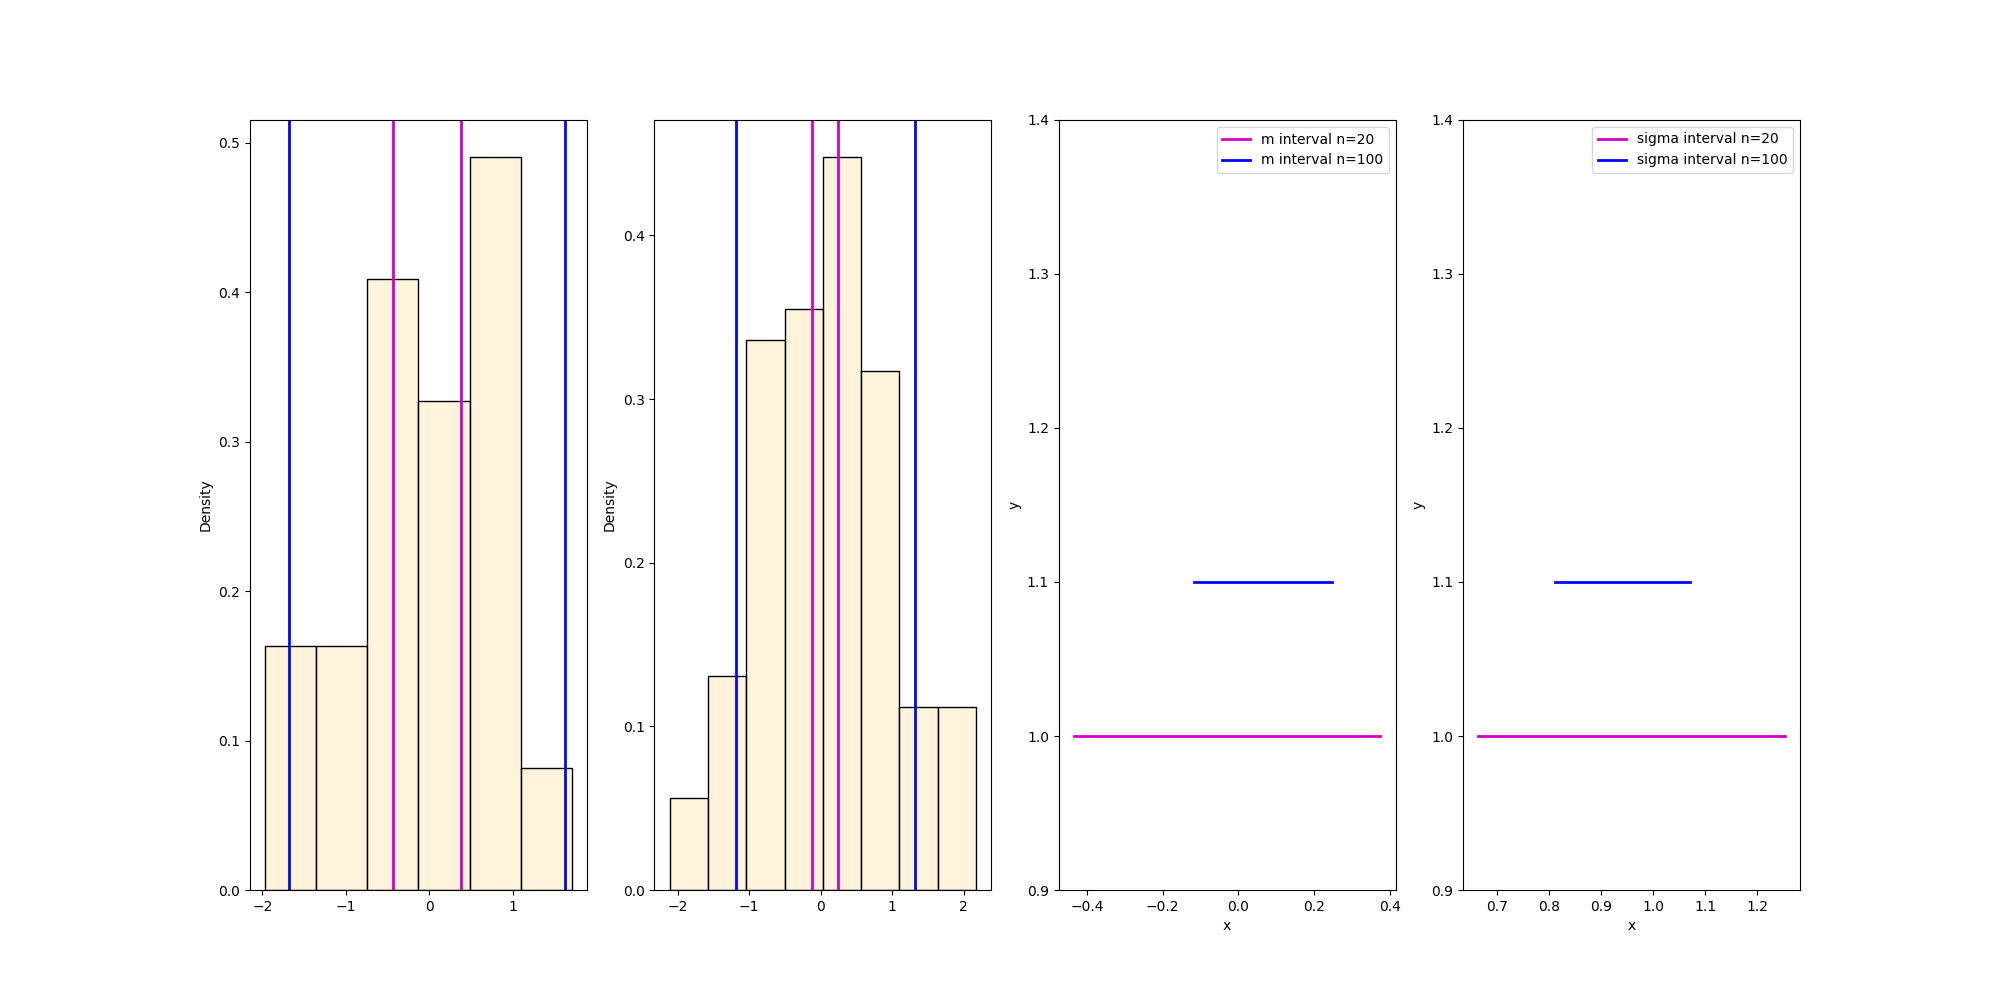
\includegraphics[width = 1.12\linewidth]{graphics/lab2_hists.png}
			\caption{Гистограммы и оценки для параметров нормального
				распределения}
		\end{center}
	\end{figure}

	\vspace{12em}

	\[
		[[-0.434162, 0.374849], [0.663480, 1.252336]]
	\]

	\[
		[[-0.117590, 0.248381], [0.810296, 1.070570]]
	\]

	\vspace{10em}

	\section{Выводы}

	По результатам выполнения лабораторной работы были сгенерированы выборки
	размером 20 и 100 элементов и построены для них боксплоты Тьюки.

	Боксплот позволяет наглядно представить основные характеристики выборки
	- медиану, квартили, межквартальный размах и выбросы. На основе
	построенных графиков можно увидеть разницу в распределении данных для
	двух выборок. Для выборки размером в 100 элементов представленные
	метрики имеют более проработанный вид, ведь с увеличением размера
	выборки улучшается точность оценок параметров распределения, но при этом
	количество выбросов растет.

	Также в ходе выполнения лабораторной работы были сгенерированы две
	выборки размерами 20 и 100 элементов для нормального и произвольного
	распределения. Затем для каждой из них были вычислены параметры
	распределения: среднее значение и дисперсия.

	Результаты, представленные графически, демонстрируют, что количество
	элементов в выборке влияет на точность оценок параметров. Более большое
	количество наблюдений (т.е. 100 элементов) приводит к более точным и
	стабильным оценкам среднего и дисперсии, как для нормального, так и для
	произвольного распределения. Для выборки с меньшим количеством элементов
	(20 элементов) оценки могут сильно варьироваться в зависимости от
	конкретной выборки, что также наглядно отображено на графиках.

	Лабораторная работа иллюстрирует важнейший статистический принцип:
	точность статистической оценки увеличивается с ростом объема выборки.
	Результаты этого исследования подчеркивают значимость использования
	достаточно больших выборок для надежного анализа данных.

	\section{Постановка задачи}

	\subsection{Коэффициент корреляции}

	Сгенерировать двумерные выборки размерами 20, 60, 100 для нормального
	двумерного распределения \( N(x, y, 0, 0, 1, 1, \rho) \). Коэффициент
	корреляции \( \rho \) взять равным 0, 0.5, 0.9. Каждая выборка
	генерируется 1000 раз и для неё вычисляются: среднее значение, среднее
	значение квадрата и дисперсия коэффициентов корреля- ции Пирсона,
	Спирмена и квадрантного коэффициента корреляции. Повторить все
	вычисления для смеси нормальных распределений:

	\[
		f(x, y) = 0.9N(x, y, 0, 0, 1, 1, 0.9) + 0.1N(x, y, 0, 0, 10, 10, -0.9).
	\]

	Изобразить сгенерированные точки на плоскости и нарисовать эллипс
	равновероятности.

	\subsection{Простая линейная регрессия}

	Найти оценки коэффициентов линейной регрессии \( y_i = a + bx_i + e_i \),
	используя 20 точек на отрезке \( [-1.8; 2] \) с равномерным шагом равным
	0.2. Ошибку \( e_i \) считать нормально распределённой с параметрами
	\( (0, 1) \). В качестве эталонной зависимости взять
	\( y_i = 2 + 2x_i + e_i \). При построении оценок коэффициентов
	использовать два критерия: критерий наименьших квадратов и критерий
	наименьших модулей. Проделать то же самое для выборки, у которой в
	значения \( y_1 \) и \( y_{20} \) вносятся возмущения 10 и -10.

	\section{Теоретическое обоснование}

	\subsection{Двумерное нормальное распределение}

	Двумерная случайная величина \( (X, Y) \) называется распределённой
	нормально (или просто нормальной), если её плотность вероятности
	определена формулой

	\begin{align} \label{eq:multivariate_normal}
		N(x, y, \bar x, \bar y, \sigma_x, \sigma_y, \rho) = \frac{1}{2 \pi \sigma_x
		\sigma_y \sqrt{1 - \rho^2}} \times \exp \left \{ -\frac{1}{2(1 - \rho^2)}
		\left [ \frac{(x - \bar x)^2}{\sigma_x^2} - 2 \rho \frac{(x - \bar x)
		(y - \bar y)}{\sigma_x \sigma_y} + \frac{(y - \bar y)^2}{\sigma_y^2}
		\right ] \right \}
	\end{align}

	Компоненты \( X \), \( Y \) двумерной нормальной случайной величины также
	распределены нормально с математическими ожиданиями \( x \), \( y \) и
	средними квадратическими отклонениями \( \sigma_x \), \( \sigma_y \)
	соответственно.

	Параметр \( \rho \) называется коэффициентом корреляции.

	\subsection{Корреляционный момент (ковариация) и коэффициент корреляции}

	Корреляционный момент, иначе ковариация, двух случайных величин \( X \) и
	\( Y \):

	\begin{equation} \label{eq:covariance}
		K = \mathbf{cov}(X, Y) = \mathbf{M}[(X - \bar x)(Y - \bar y)]
	\end{equation}

	Коэффициент корреляции \( \rho \) двух случайных величин \( X \) и
	\( Y \):

	\begin{equation} \label{eq:correlation}
		\rho = \frac{K}{\sigma_x \sigma_y}
	\end{equation}

	\subsection{Выборочный коэффициент корреляции Пирсона}

	Выборочный коэффициент корреляции Пирсона:

	\begin{equation} \label{eq:pearson_corr}
		r = \frac{\frac{1}{n} \sum (x_i - \bar x)(y_i - \bar y)}{\sqrt{\frac{1}{n}
		\sum (x_i - \bar x)^2 \frac{1}{n} \sum (y_i - \bar y)^2}} =
		\frac{K}{s_X s_Y},
	\end{equation}

	где \( K \), \( s_X^2 \), \( x_Y^2 \) — выборочные ковариации и дисперсии
	случайных величин \( X \) и \( Y \).

	\subsection{Выборочный квадрантный коэффициент корреляции}

	Выборочный квадрантный коэффициент корреляции

	\begin{equation} \label{eq:quadrant_corr}
		r_Q = \frac{(n_1 + n_3) - (n_2 + n_4)}{n},
	\end{equation}

	где \( n_1 \), \( n_2 \), \( n_3 \), \( n_4 \) — количество точек с
	координатами \( (x_i, y_i) \), попавшими, соответственно, в I, II, III, IV
	квадранты декартовой системы с осями \( x' = x - \mathbf{med}x \),
	\( y' = y - \mathbf{med}y \).

	\subsection{Выборочный коэффициент ранговой корреляции Спирмена}

	Обозначим ранги, соотвествующие значениям переменной \( X \), через
	\( u \), а ранги, соотвествующие значениям переменной \( Y \), — через
	\( v \).

	Выборочный коэффициент ранговой корреляции Спирмена:

	\begin{equation}  \label{eq:spearman_corr}
		r_S = \frac{\frac{1}{n} \sum (u_i - \bar u)(v_i - \bar v)}{\sqrt{\frac{1}{n}
		\sum (u_i - \bar u)^2 \frac{1}{n} \sum (v_i - \bar v)^2}},
	\end{equation}

	где \( \bar u = \bar v = \frac{1 + 2 + \dots + n}{n} = \frac{n + 1}{2} \) —
	среднее значение рангов.

	\subsection{Эллипсы рассеивания}

	Уравнение проекции эллипса рассеивания на плоскость \( xOy \):

	\begin{equation}  \label{eq:ellipse}
		\frac{(x - \bar x)^2}{\sigma_x^2} - 2 \rho \frac{(x - \bar x)(y - \bar y)}
		{\sigma_x \sigma_y} + \frac{(y - \bar y)^2}{\sigma_y^2} = \text{const}.
	\end{equation}

	Центр эллипса \ref{eq:ellipse} находится в точке с координатами
	\( (x, y) \); оси симметрии эллипса составляют с осью \( Ox \) углы,
	определяемые уравнением

	\begin{equation}  \label{eq:ellipse}
		\tg 2 \alpha = \frac{2 \rho \sigma_x \sigma_y}{\sigma_x^2 - \sigma_y^2}.
	\end{equation}

	\subsection{Метод наименьших квадратов}

	При оценивании параметров регрессионной модели используют различные
	методы. Один из наиболее распрстранённых подходов заключается в
	следующем: вводится мера (критерий) рассогласования отклика и
	регрессионной функции, и оценки параметров регрессии определяются так,
	чтобы сделать это рассогласование наименьшим. Достаточно простые
	расчётные формулы для оценок получают при выборе критерия в виде суммы
	квадратов отклонений значений отклика от значений регрессионной функции
	(сумма квадратов остатков):

	\begin{equation} \label{eq:lsm}
		Q(\beta_0, \beta_1) = \sum \limits_{i=1}^n \varepsilon_i^2 =
		\sum \limits_{i=1}^n (y_i - \beta_0 - \beta_1 x_i)^2 \rightarrow
		\min_{\beta_0, \beta_1}.
	\end{equation}

	Задача минимизации квадратичного критерия \eqref{eq:lsm} носит название
	задачи метода наименьших квадратов (МНК), а оценки \( \beta_0 \),
	\( \beta_1 \) параметров \( \beta_0 \), \( \beta_1 \), реализующие минимум
	критерия \eqref{eq:lsm}, называют МНК-оценками.

	\subsection{Метод наименьших модулей}

	Робастность оценок коэффициентов линейной регрессии (т.е. их
	устойчивость по отношению к наличию в данных редких, но больших по
	величине выбросов) может быть обеспечена различными способами. Одним из
	них является использование метода наименьших модулей вместо метода
	наименьших квадратов:

	\begin{equation} \label{eq:lam}
		\sum \limits_{i=1}^n |y_i - \beta_0 - \beta_1 x_i| \rightarrow
		\min_{\beta_0, \beta_1}.
	\end{equation}


	\section{Описание работы}
	Лабораторные работы выполнены с использованием Python и его сторонних
	библиотек \verb!numpy!, \verb!pandas!, \verb!matplotlib!, \verb!seaborn! были
	построены гистограммы распределений и посчитаны характеристики пложения.

	Ссылка на GitHub репозиторий:
	\href{https://github.com/vladimir-skvortsov/spbstu-mathematical-statistics}
	{https://github.com/vladimir-skvortsov/spbstu-mathematical-statistics}

	\section{Результаты}

	\subsection{Коэффициент корреляции}

	\begin{table}[htbp!]
		\centering
		\begin{tabular}{ |c|c|c|c| }
			\hline
			\( n = 20 \), \( \rho = 0 \) & & & \\
			\hline
			& \( r \) \eqref{eq:pearson_corr} & \( r_S \) \eqref{eq:spearman_corr} &
			\( r_Q \) \eqref{eq:quadrant_corr} \\
			\hline
			Среднее & \( 8.051 \times 10^{-3} \) & \( 8.633 \times 10^{-3} \) &
			\( 1.216 \times 10^{-2} \) \\
			\hline
			Среднее квадратов & \( 5.501 \times 10^{-2} \) &
			\( 5.418 \times 10^{-2} \) & \( 1.033 \times 10^{-1} \) \\
			\hline
			Дисперсия & \( 5.495 \times 10^{-2} \) &
			\( 5.410 \times 10^{-2} \) & \( 1.031 \times 10^{-1} \) \\
			\hline
			\hline
			\( n = 20 \), \( \rho = 0.5 \) & & & \\
			\hline
			& \( r \) \eqref{eq:pearson_corr} & \( r_S \) \eqref{eq:spearman_corr} &
			\( r_Q \) \eqref{eq:quadrant_corr} \\
			\hline
			Среднее & \( 4.933 \times 10^{-1} \) & \( 4.674 \times 10^{-1} \) &
			\( 4.644 \times 10^{-1} \) \\
			\hline
			Среднее квадратов & \( 2.743 \times 10^{-1} \) &
			\( 2.534 \times 10^{-1} \) & \( 3.139 \times 10^{-1} \) \\
			\hline
			Дисперсия & \( 3.093 \times 10^{-2} \) &
			\( 3.496 \times 10^{-2} \) & \( 9.823 \times 10^{-2} \) \\
			\hline
			\hline
			\( n = 20 \), \( \rho = 0.9 \) & & & \\
			\hline
			& \( r \) \eqref{eq:pearson_corr} & \( r_S \) \eqref{eq:spearman_corr} &
			\( r_Q \) \eqref{eq:quadrant_corr} \\
			\hline
			Среднее & \( 8.938 \times 10^{-1} \) & \( 8.646 \times 10^{-1} \) &
			\( 9.837 \times 10^{-1} \) \\
			\hline
			Среднее квадратов & \( 8.014 \times 10^{-1} \) &
			\( 7.527 \times 10^{-1} \) & \( 1.026 \) \\
			\hline
			Дисперсия & \( 2.454 \times 10^{-3} \) &
			\( 5.209 \times 10^{-3} \) & \( 5.804 \times 10^{-2} \) \\
			\hline
			\hline
			\( n = 60 \), \( \rho = 0 \) & & & \\
			\hline
			& \( r \) \eqref{eq:pearson_corr} & \( r_S \) \eqref{eq:spearman_corr} &
			\( r_Q \) \eqref{eq:quadrant_corr} \\
			\hline
			Среднее & \( 8.143 \times 10^{-3} \) & \( 8.747 \times 10^{-3} \) &
			\( 8.485 \times 10^{-3} \) \\
			\hline
			Среднее квадратов & \( 1.709 \times 10^{-2} \) &
			\( 1.689 \times 10^{-2} \) & \( 3.111 \times 10^{-2} \) \\
			\hline
			Дисперсия & \( 1.703 \times 10^{-2} \) &
			\( 1.682 \times 10^{-2} \) & \( 3.104 \times 10^{-2} \) \\
			\hline
			\hline
			\( n = 60 \), \( \rho = 0.5 \) & & & \\
			\hline
			& \( r \) \eqref{eq:pearson_corr} & \( r_S \) \eqref{eq:spearman_corr} &
			\( r_Q \) \eqref{eq:quadrant_corr} \\
			\hline
			Среднее & \( 4.985 \times 10^{-1} \) & \( 4.757 \times 10^{-1} \) &
			\( 4.668 \times 10^{-1} \) \\
			\hline
			Среднее квадратов & \( 2.585 \times 10^{-1} \) &
			\( 2.373 \times 10^{-1} \) & \( 2.504 \times 10^{-1} \) \\
			\hline
			Дисперсия & \( 1.000 \times 10^{-2} \) &
			\( 1.094 \times 10^{-2} \) & \( 3.256 \times 10^{-2} \) \\
			\hline
			\hline
			\( n = 60 \), \( \rho = 0.9 \) & & & \\
			\hline
			& \( r \) \eqref{eq:pearson_corr} & \( r_S \) \eqref{eq:spearman_corr} &
			\( r_Q \) \eqref{eq:quadrant_corr} \\
			\hline
			Среднее & \( 8.979 \times 10^{-1} \) & \( 8.810 \times 10^{-1} \) &
			\( 9.937 \times 10^{-1} \) \\
			\hline
			Среднее квадратов & \( 8.069 \times 10^{-1} \) &
			\( 7.774 \times 10^{-1} \) & \( 1.004 \) \\
			\hline
			Дисперсия & \( 7.297 \times 10^{-4} \) &
			\( 1.202 \times 10^{-3} \) & \( 1.700 \times 10^{-2} \) \\
			\hline
			\hline
			\( n = 100 \), \( \rho = 0 \) & & & \\
			\hline
			& \( r \) \eqref{eq:pearson_corr} & \( r_S \) \eqref{eq:spearman_corr} &
			\( r_Q \) \eqref{eq:quadrant_corr} \\
			\hline
			Среднее & \( 1.396 \times 10^{-3} \) & \( 8.326 \times 10^{-5} \) &
			\( 1.584 \times 10^{-3} \) \\
			\hline
			Среднее квадратов & \( 9.856 \times 10^{-3} \) &
			\( 9.848 \times 10^{-3} \) & \( 1.972 \times 10^{-2} \) \\
			\hline
			Дисперсия & \( 9.854 \times 10^{-3} \) &
			\( 9.848 \times 10^{-3} \) & \( 1.972 \times 10^{-2} \) \\
			\hline
			\hline
			\( n = 100 \), \( \rho = 0.5 \) & & & \\
			\hline
			& \( r \) \eqref{eq:pearson_corr} & \( r_S \) \eqref{eq:spearman_corr} &
			\( r_Q \) \eqref{eq:quadrant_corr} \\
			\hline
			Среднее & \( 5.013 \times 10^{-1} \) & \( 4.812 \times 10^{-1} \) &
			\( 4.723 \times 10^{-1} \) \\
			\hline
			Среднее квадратов & \( 2.568 \times 10^{-1} \) &
			\( 2.375 \times 10^{-1} \) & \( 2.407 \times 10^{-1} \) \\
			\hline
			Дисперсия & \( 5.481 \times 10^{-3} \) &
			\( 6.013 \times 10^{-3} \) & \( 1.762 \times 10^{-2} \) \\
			\hline
			\hline
			\( n = 100 \), \( \rho = 0.9 \) & & & \\
			\hline
			& \( r \) \eqref{eq:pearson_corr} & \( r_S \) \eqref{eq:spearman_corr} &
			\( r_Q \) \eqref{eq:quadrant_corr} \\
			\hline
			Среднее & \( 8.999 \times 10^{-1} \) & \( 8.866 \times 10^{-1} \) &
			\( 1.003 \) \\
			\hline
			Среднее квадратов & \( 8.103 \times 10^{-1} \) &
			\( 7.868 \times 10^{-1} \) & \( 1.017 \) \\
			\hline
			Дисперсия & \( 4.017 \times 10^{-4} \) &
			\( 6.665 \times 10^{-4} \) & \( 1.049 \times 10^{-2} \) \\
			\hline
		\end{tabular}
		\caption{Характеристики нормального двумерного распределения}
	\end{table}

	\begin{table}[htbp!]
		\centering
		\begin{tabular}{ |c|c|c|c| }
			\hline
			\( n = 20 \) & & & \\
			\hline
			& \( r \) \eqref{eq:pearson_corr} & \( r_S \) \eqref{eq:spearman_corr} &
			\( r_Q \) \eqref{eq:quadrant_corr} \\
			\hline
			Среднее & \( -7.987 \times 10^{-2} \) & \( -7.020 \times 10^{-2} \) &
			\( -6.336 \times 10^{-2} \) \\
			\hline
			Среднее квадратов & \( 5.968 \times 10^{-2} \) &
			\( 5.944 \times 10^{-2} \) & \( 1.112 \times 10^{-1} \) \\
			\hline
			Дисперсия & \( 5.330 \times 10^{-2} \) &
			\( 5.451 \times 10^{-2} \) & \( 1.072 \times 10^{-1} \) \\
			\hline
			\hline
			\( n = 60 \) & & & \\
			\hline
			& \( r \) \eqref{eq:pearson_corr} & \( r_S \) \eqref{eq:spearman_corr} &
			\( r_Q \) \eqref{eq:quadrant_corr} \\
			\hline
			Среднее & \( 9.290 \times 10^{-2} \) & \( -8.988 \times 10^{-2} \) &
			\( -8.730 \times 10^{-2} \) \\
			\hline
			Среднее квадратов & \( 2.606 \times 10^{-2} \) &
			\( 2.553 \times 10^{-2} \) & \( 4.290 \times 10^{-2} \) \\
			\hline
			Дисперсия & \( 1.743 \times 10^{-2} \) &
			\( 1.745 \times 10^{-2} \) & \( 3.528 \times 10^{-2} \) \\
			\hline
			\hline
			\( n = 100 \) & & & \\
			\hline
			& \( r \) \eqref{eq:pearson_corr} & \( r_S \) \eqref{eq:spearman_corr} &
			\( r_Q \) \eqref{eq:quadrant_corr} \\
			\hline
			Среднее & \( -1.013 \times 10^{-1} \) & \( -9.639 \times 10^{-2} \) &
			\( -9.011 \times 10^{-2} \) \\
			\hline
			Среднее квадратов & \( 2.047 \times 10^{-2} \) &
			\( 1.984 \times 10^{-2} \) & \( 2.968 \times 10^{-2} \) \\
			\hline
			Дисперсия & \( 1.021 \times 10^{-2} \) &
			\( 1.054 \times 10^{-2} \) & \( 2.156 \times 10^{-2} \) \\
			\hline
		\end{tabular}
		\caption{Характеристики смеси нормальных распределений}
	\end{table}

	\begin{figure}[htbp!]
		\begin{center}
			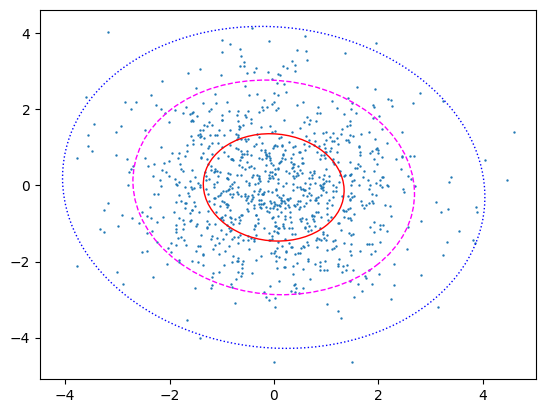
\includegraphics[width = 0.8\linewidth]{graphics/lab5_ellips_1.png}
			\caption{Смесь нормальных распределений и эллипсы равновероятности
			( \( \rho = 0 \) )}
		\end{center}
	\end{figure}

	\begin{figure}[htbp!]
		\begin{center}
			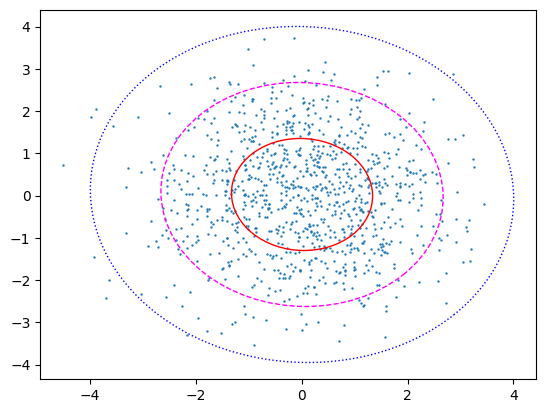
\includegraphics[width = 0.8\linewidth]{graphics/lab5_ellips_2.png}
			\caption{Смесь нормальных распределений и эллипсы равновероятности
			( \( \rho = 0.5 \) )}
		\end{center}
	\end{figure}

	\begin{figure}[htbp!]
		\begin{center}
			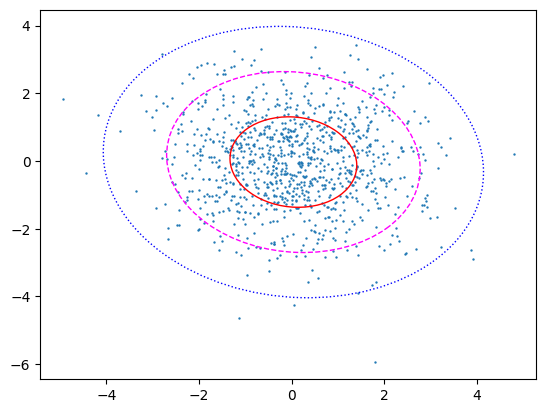
\includegraphics[width = 0.8\linewidth]{graphics/lab5_ellips_3.png}
			\caption{Смесь нормальных распределений и эллипсы равновероятности
			( \( \rho = 0.9 \) )}
		\end{center}
	\end{figure}

	\clearpage

	\subsection{Простая линейная регрессия}

	\begin{figure}[htbp!]
		\begin{center}
			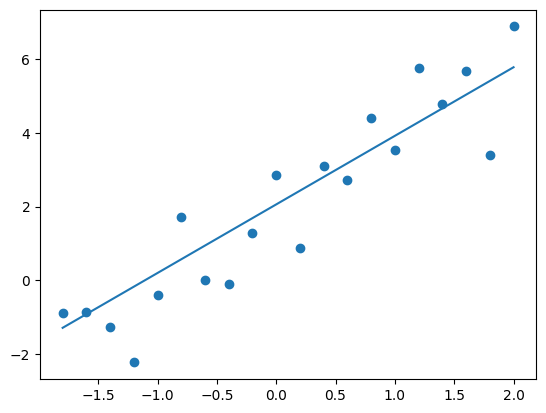
\includegraphics[width = 1\linewidth]{graphics/lab6_sq.png}
			\caption{Метод наименьших квадратов \( ( 1.861, 2.061) \)}
		\end{center}
	\end{figure}

	\begin{figure}[htbp!]
		\begin{center}
			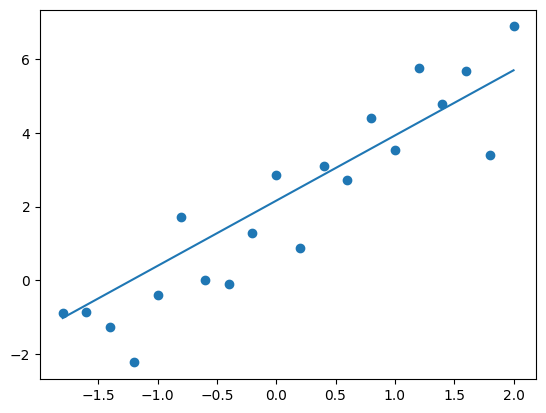
\includegraphics[width = 1\linewidth]{graphics/lab6_abs.png}
			\caption{Метод наименьших модулей \( (1.7691, 2.162) \)}
		\end{center}
	\end{figure}

	\begin{figure}[htbp!]
		\begin{center}
			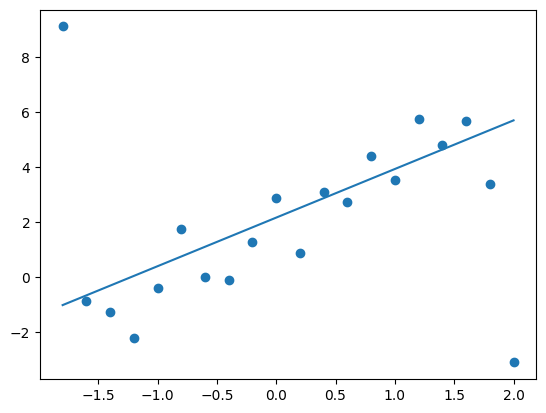
\includegraphics[width = 1\linewidth]{graphics/lab6_abs_mod.png}
			\caption{Метод наименьших квадратов с возмущениями
				\( (1.668, 1.990) \)}
		\end{center}
	\end{figure}

	\begin{figure}[htbp!]
		\begin{center}
			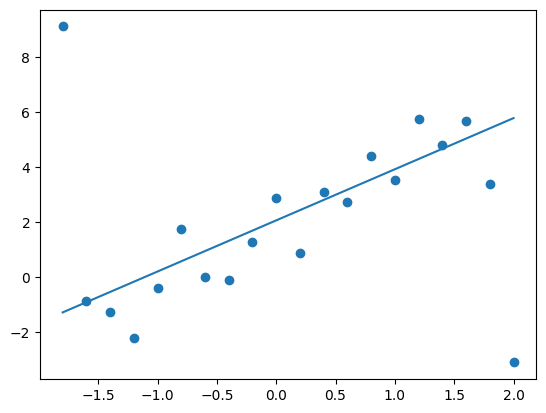
\includegraphics[width = 1\linewidth]{graphics/lab6_sq_mod.png}
			\caption{Метод наименьших модулей с возмущениями \( (2.004, 0.632) \)}
		\end{center}
	\end{figure}

	\clearpage

	\section{Выводы}

	На основе полученных характеристик (включая среднее значение, среднее
	значение квадрата и дисперсию) для различных коэффициентов корреляции и
	размеров выборки, можно сделать следующие наблюдения:

	\begin{enumerate}
		\item При увеличении размера выборки повышается точность оценок, что
		видно по уменьшению дисперсий коэффициентов корреляции. Это
		соответствует принципам центральной предельной теоремы и закона
		больших чисел.
		\item При увеличении коэффициента корреляции \( \rho \), средние
		значения коэффициентов Пирсона, Спирмена и квадратичного коэффициента
		корреляции тоже увеличиваются. Это указывает на прямую связь между
		\( \rho \) и другими коэффициентами корреляции.
	\end{enumerate}

	Из результатов оценок коэффициентов линейной регрессии при использовании
	двух критериев (критерий наименьших квадратов и критерий наименьших
	модулей) можно сделать следующие выводы:

	\begin{enumerate}
		\item Метод наименьших квадратов показал себя эффективно в случае,
		когда нет значительных выбросов в данных, в то время как метод
		наименьших модулей проявил себя лучше в присутствии значительных
		возмущений.
		\item Важно выбирать метод, исходя из особенностей данных. Если в
		данных присутствуют выбросы, метод наименьших модулей будет
		предпочтительнее из-за его устойчивости к выбросам.
	\end{enumerate}
\end{document}
